\documentclass[letterpaper,12pt]{article}
\usepackage[margin=1in]{geometry}
\usepackage{xltxtra}
\setmainfont[Mapping=tex-text]{Liberation Serif}
\setmonofont[Scale=0.8]{Liberation Mono}
\newcommand{\var}[1]{\texttt{\$\{#1\}}}
\usepackage[colorlinks=false,pdfborder=0 0 0]{hyperref}
\usepackage{graphicx}

\title{Instalog Requirements Specification}
\author{
Billy R. O'Neal III (bro4@case.edu) \\
Jacob Snyder (jrs213@case.edu)
}

\begin{document}

\maketitle

\section{Introduction}
Instalog is a senior project by Jacob Snyder and Billy O'Neal, which is designed
to gather information from Microsoft Windows installations, for the purpose of
malware removal and system repair.  It must generate a human and machine
readable report which assists end users, remote experts, and local
administrators with issue diagnosis and malware removal.

Instalog is inspired by several similar tools which all share some basic
functionality.  In many ways, Instalog can be viewed as an evolution of
these tools:
\begin{itemize}
    \item TrendMicro's {\em Hijack This} (HJT)
    \item ``sUBs'' {\em Doesn't Do Squat} (DDS)
    \item ``random/random'''s {\em Random's System Information Tool} (RSIT)
    \item ``OldTimer'''s {\em OTA}, {\em OTS}, and {\em OTL} (formerly
    OTAnalyzeIt, OTScanIt, and OTListIt, respectively)
    \item Sysinternals' {\em Autoruns}
    \item Runscanner's {\em Runscanner}
\end{itemize}
all of which purport to accomplish similar goals to Instalog. However, each of
these tools has bugs or specific behavior which cause problems for at least one
of Instalog's three intended user groups.

Specifically, the above tools contain one or more of the above problems:
\begin{itemize}
    \item Incorrect handling and escaping of log data
    \item Lack of published specifications, documentation, or source code
    \item Outstanding bugs that the authors are unwilling or unable to fix
    \item Lack of scriptability, for the purposes of modifying log output and
    malware removal.
    \item Lack of 64 bit support.
    \item Lack of Unicode support.
    \item Lack of enumeration of some types of useful log information.
\end{itemize}
Instalog will attempt to solve those problems by combining characteristics of
the above tools which are deemed useful, while mixing in a few tricks of it's
own.

\subsection{Document Conventions}
Within the scope of this document, computer output or other information that is
to be taken literally is written in \texttt{fixed width text}. In some
instances, a block of fixed width text will be surrouned by non-fixed width
quotes ``\texttt{ like this}''. In such cases, the quotes are not significant,
and there will there will (typically) be leading or trailing space around the
fixed width block, which is significant and MUST NOT be removed. Variables,
which are replaced with some content, are written of the form \var{name}, and
will be explained in greater detail in prose surrounding a given block of
\texttt{fixed width} text.

\subsection{Intended Audience}
Instalog is designed with three types of target users in mind. These ``user
classes'' are listed in the following sections.

\subsubsection{Home Users}
For a typical home user, Instalog MUST NOT display a complicated interface, and
must make it relatively difficult to misstep and take a wrong action. Few
options need be presented, such as the ability to generate a default report and
the ability to take a given script and run it on a target machine. Complicated
features such as analysis MUST NOT be displayed; though they may appear as
options that are, by default, deselected.

\subsubsection{Administrators}
Administrators are similar to home users in that they are physically working at
a computer being examined, but they are different in that they have the inten of
repairing their own computer or the computer of a client. They wish to see
analysis features and more possible options. Instalog MUST provide a means for
Administrators to use it's analysis features without manual saving and reloading
of log files.

\subsubsection{Forum Experts}
Forum Experts help typical end users repair their machines remotely over
self-help forums such as BleepingComputer.com or GeeksToGo.com.
These users work remotely, and likely will never see a given target
machine.
Instalog MUST produce log formats that are human readable in the vast majority
of cases, but which can be passed through common forum software such as Invision
Power Board, phpBB, or vBulletin without destruction of information.
Unforunately, this makes common data exchange formats such as JSON and XML
unsuitable. 

Moreover, as obtaining additional information from a machine may
have lead times of several days, Instalog's report must be unambiguous; that is,
no two possible system configurations may produce the same output. Experts can
also benefit from log analysis features. Finally, Experts need to be able to
write simple, human readable scripts to perform actions to fix a user's machine
remotely.

\subsection{Acknowledgements}
Instalog's authors would like to thank ``sUBs'' for use of DDS's whitelisting
data for use in Instalog, and for being available for occasonal clarification
of problems. He also allowed use of a modified form of DDS' logging format.

Instalog also was constructed with feedback taken from self help forums like
BleepingComputer, and students in Dr. Glutekin Özsoyoğlu's EECS 395: Senior
Project class of Spring 2012, at Case Western Reserve University.

\subsection{Licensing} \label{sec:licensing}
Instalog itself is to be released under the two clause form of the BSD license,
which is reprinted below:

\begin{verbatim}
Copyright © 2012, Jacob Snyder, Billy O'Neal III, and "sUBs"
All rights reserved.

Redistribution and use in source and binary forms, with or without
modification, are permitted provided that the following conditions are met: 

1. Redistributions of source code must retain the above copyright notice, this
   list of conditions and the following disclaimer. 
2. Redistributions in binary form must reproduce the above copyright notice,
   this list of conditions and the following disclaimer in the documentation
   and/or other materials provided with the distribution. 

THIS SOFTWARE IS PROVIDED BY THE COPYRIGHT HOLDERS AND CONTRIBUTORS "AS IS" AND
ANY EXPRESS OR IMPLIED WARRANTIES, INCLUDING, BUT NOT LIMITED TO, THE IMPLIED
WARRANTIES OF MERCHANTABILITY AND FITNESS FOR A PARTICULAR PURPOSE ARE
DISCLAIMED. IN NO EVENT SHALL THE COPYRIGHT OWNER OR CONTRIBUTORS BE LIABLE FOR
ANY DIRECT, INDIRECT, INCIDENTAL, SPECIAL, EXEMPLARY, OR CONSEQUENTIAL DAMAGES
(INCLUDING, BUT NOT LIMITED TO, PROCUREMENT OF SUBSTITUTE GOODS OR SERVICES;
LOSS OF USE, DATA, OR PROFITS; OR BUSINESS INTERRUPTION) HOWEVER CAUSED AND
ON ANY THEORY OF LIABILITY, WHETHER IN CONTRACT, STRICT LIABILITY, OR TORT
(INCLUDING NEGLIGENCE OR OTHERWISE) ARISING IN ANY WAY OUT OF THE USE OF THIS
SOFTWARE, EVEN IF ADVISED OF THE POSSIBILITY OF SUCH DAMAGE.
\end{verbatim}

This document, along with all other documentation related to Instalog,  is to be
released under the Creative Commons Attrribution 3.0 Unported license. Human
readable and lawyer readable versions of this license can be found at
\url{http://creativecommons.org/licenses/by/3.0/}.

\subsection{Minimum System Requirements}
Instalog MUST run on all Microsoft Windows NT variants released later than
Windows 2000 (x86, SP4 only). This includes all versions Windows XP (x86 and
x64, RTM, SP1, SP2, and SP3 (on x86 machines)), Windows Vista (x86 and x64, RTM,
SP1, and SP2), Windows 7 (x86 and x64, RTM and SP1), Windows Server 2003 (x86
and x64, RTM, SP1, and SP2), Windows Server 2003 R2 (x86 and x64, RTM, SP1, and
SP2), Windows Server 2008 (x86 and x64, RTM, SP1, and SP2), Windows Server 2008
R2 (x64, RTM, and SP1).

No attempt will be made to support Itanium architecture systems as Instalog's
authors do not have access to suitable testing hardware. No attempt will be made
to support MS-DOS based versions of Windows. Instalog's behavior on unsupported
machines must not cause data destruction, but is otherwise undefined.

\section{Graphical User Interface}
The Graphical User Interface (GUI) is designed in such a way that it can
accommodate the various usage scenarios common for this tool.  Therefore, it
must bridge the gap between simplicity and complexity so that users can simply
use the tool and power users can use the tool to create powerful system-altering
scripts.

The GUI is inspired by the well-known Windows application installer paradigm. 
Basic users will only encounter screens similar to what they are familiar with
when installing or uninstalling applications.  The interface will become much
more complex when power users use the tool to modify scripts, but this is to be
expected.  The editing script interface is inspired by tools that exist in the
field (namely OTA and HijackThis).

\subsection{Main}
When a user opens the application, they must be presented with the screen from
Figure~\ref{fig:gui_main}.  This screen is the decision point of the
application.  Depending on the user's input, this screen will take the user
through the workflows of this tool.

\begin{figure}[h]
  	\centering
	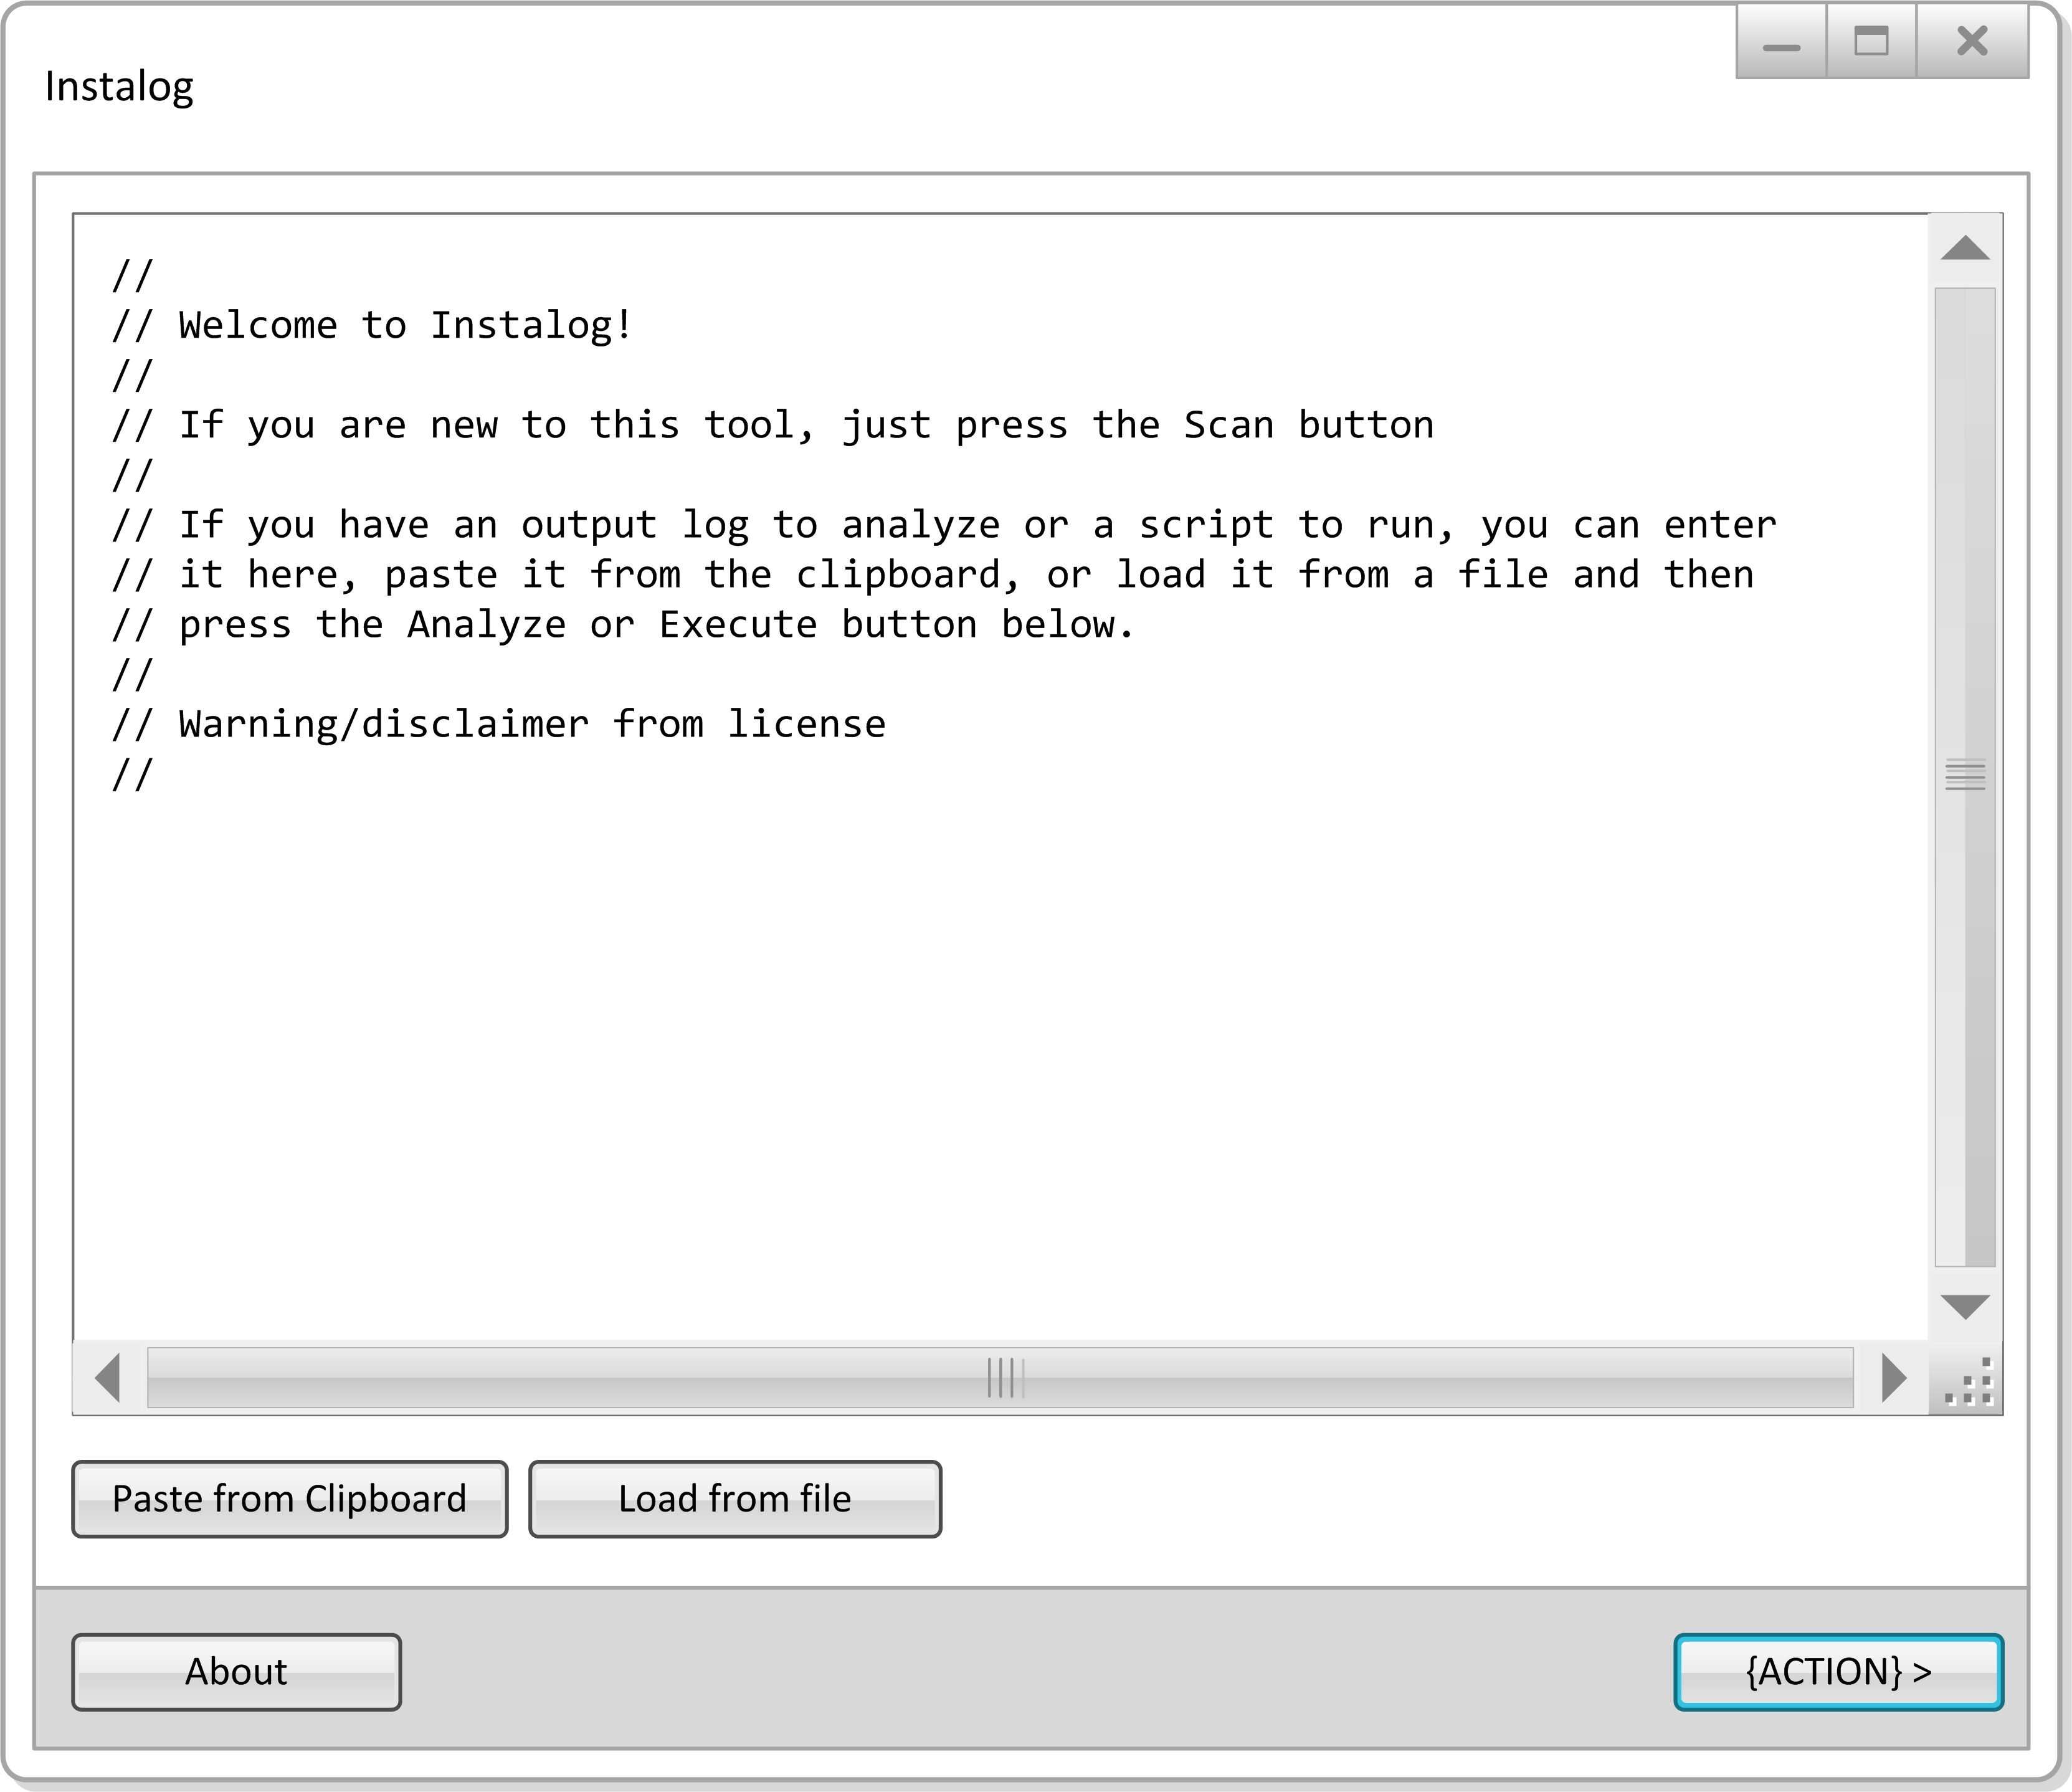
\includegraphics{figures/gui/Main.png}
  	\caption{GUI Main Screen}
  	\label{fig:gui_main}
\end{figure}

\begin{description}
\item[Textbox requirements] \hfill
\begin{enumerate}
\item The textbox shall support basic operations including but not limited to
Copy, Paste, and Undo/Redo.
\item Thee textbox shall not implement word-wrap.	  
\end{enumerate}

\item[Paste from Clipboard button requirements] \hfill
\begin{enumerate}
\item This button shall clear the contents of the textbox and then place
the full contents of the clipboard into the textbox
\item If the clipboard does not contain text data, this button must be
disabled
\end{enumerate}

\item[Load from File button requirements] \hfill
\begin{enumerate}
\item Pressing this button will the standard Windows file open dialog.  It
shall be enabled for searching for \texttt{*.txt} and \texttt{*.zip} files.
\begin{enumerate}
\item  If a valid file is opened, the contents of the textbox shall be cleared
and then the full contents of the file shall be placed into the textbox.
Obviously, zipped files should be unzipped.
\item If the user presses cancel in the dialog, the contents of the textbox
shall not be changed
\end{enumerate}
\end{enumerate}

\item[\var{action} button requirements] \hfill
\begin{enumerate}
\item The contents of the textbox shall be scanned to determine if it contains
default script content (or empty script content), script content, or log
content.  If so, the button shall display ``Scan," ``Execute," or ``Analyze"
(respectively).
\item The button shall have differing behavior based on the inferred content of
the textbox:
\begin{enumerate}
\item If the button reads ``Scan," the tool shall proceed to the Running Screen
(section~\ref{sec:running_screen}) running the default script
(section~\ref{sec:default_script_sections}).
\item If the button reads ``Execute," the tool shall proceed to the Running
Screen (section~\ref{sec:running_screen}) running the supplied script.
\item If the button reads ``Analyze," the tool shall proceed to the Analysis
Screen (section~\ref{sec:analysis_screen}) displaying the parsed log.
\end{enumerate}
\item If the type of the content in the textbox cannot be inferred or the
content of the textbox is not syntactically valid, the button shall display
the text of the last inferred \var{ACTION}.  If the user presses the
\var{ACTION} button for an invalid script, the application must not continue. 
Instead, an error message must appear that informs the user that the script is
invalid and therefore the tool will not continue.
\end{enumerate}

\item[About button requirements] \hfill
\begin{enumerate}
\item This button shall display a screen that contains the license for this
project (section~\ref{sec:licensing}) as well as information for any other
tools used in this project.  This screen shall have a simple close button.
\item The behavior for this button is the same on all following windows. 
\end{enumerate}
\end{description}

\subsection{Running Screen} \label{sec:running_screen}
This screen will run a script.  For the purpose of these requirements, it is not
important whether the script is the default script or a custom script.  The
script shall automatically begin when this screen is displayed.  The Running 
Screen is presented in Figure~\ref{fig:gui_running}.

\begin{figure}[h]
  	\centering
	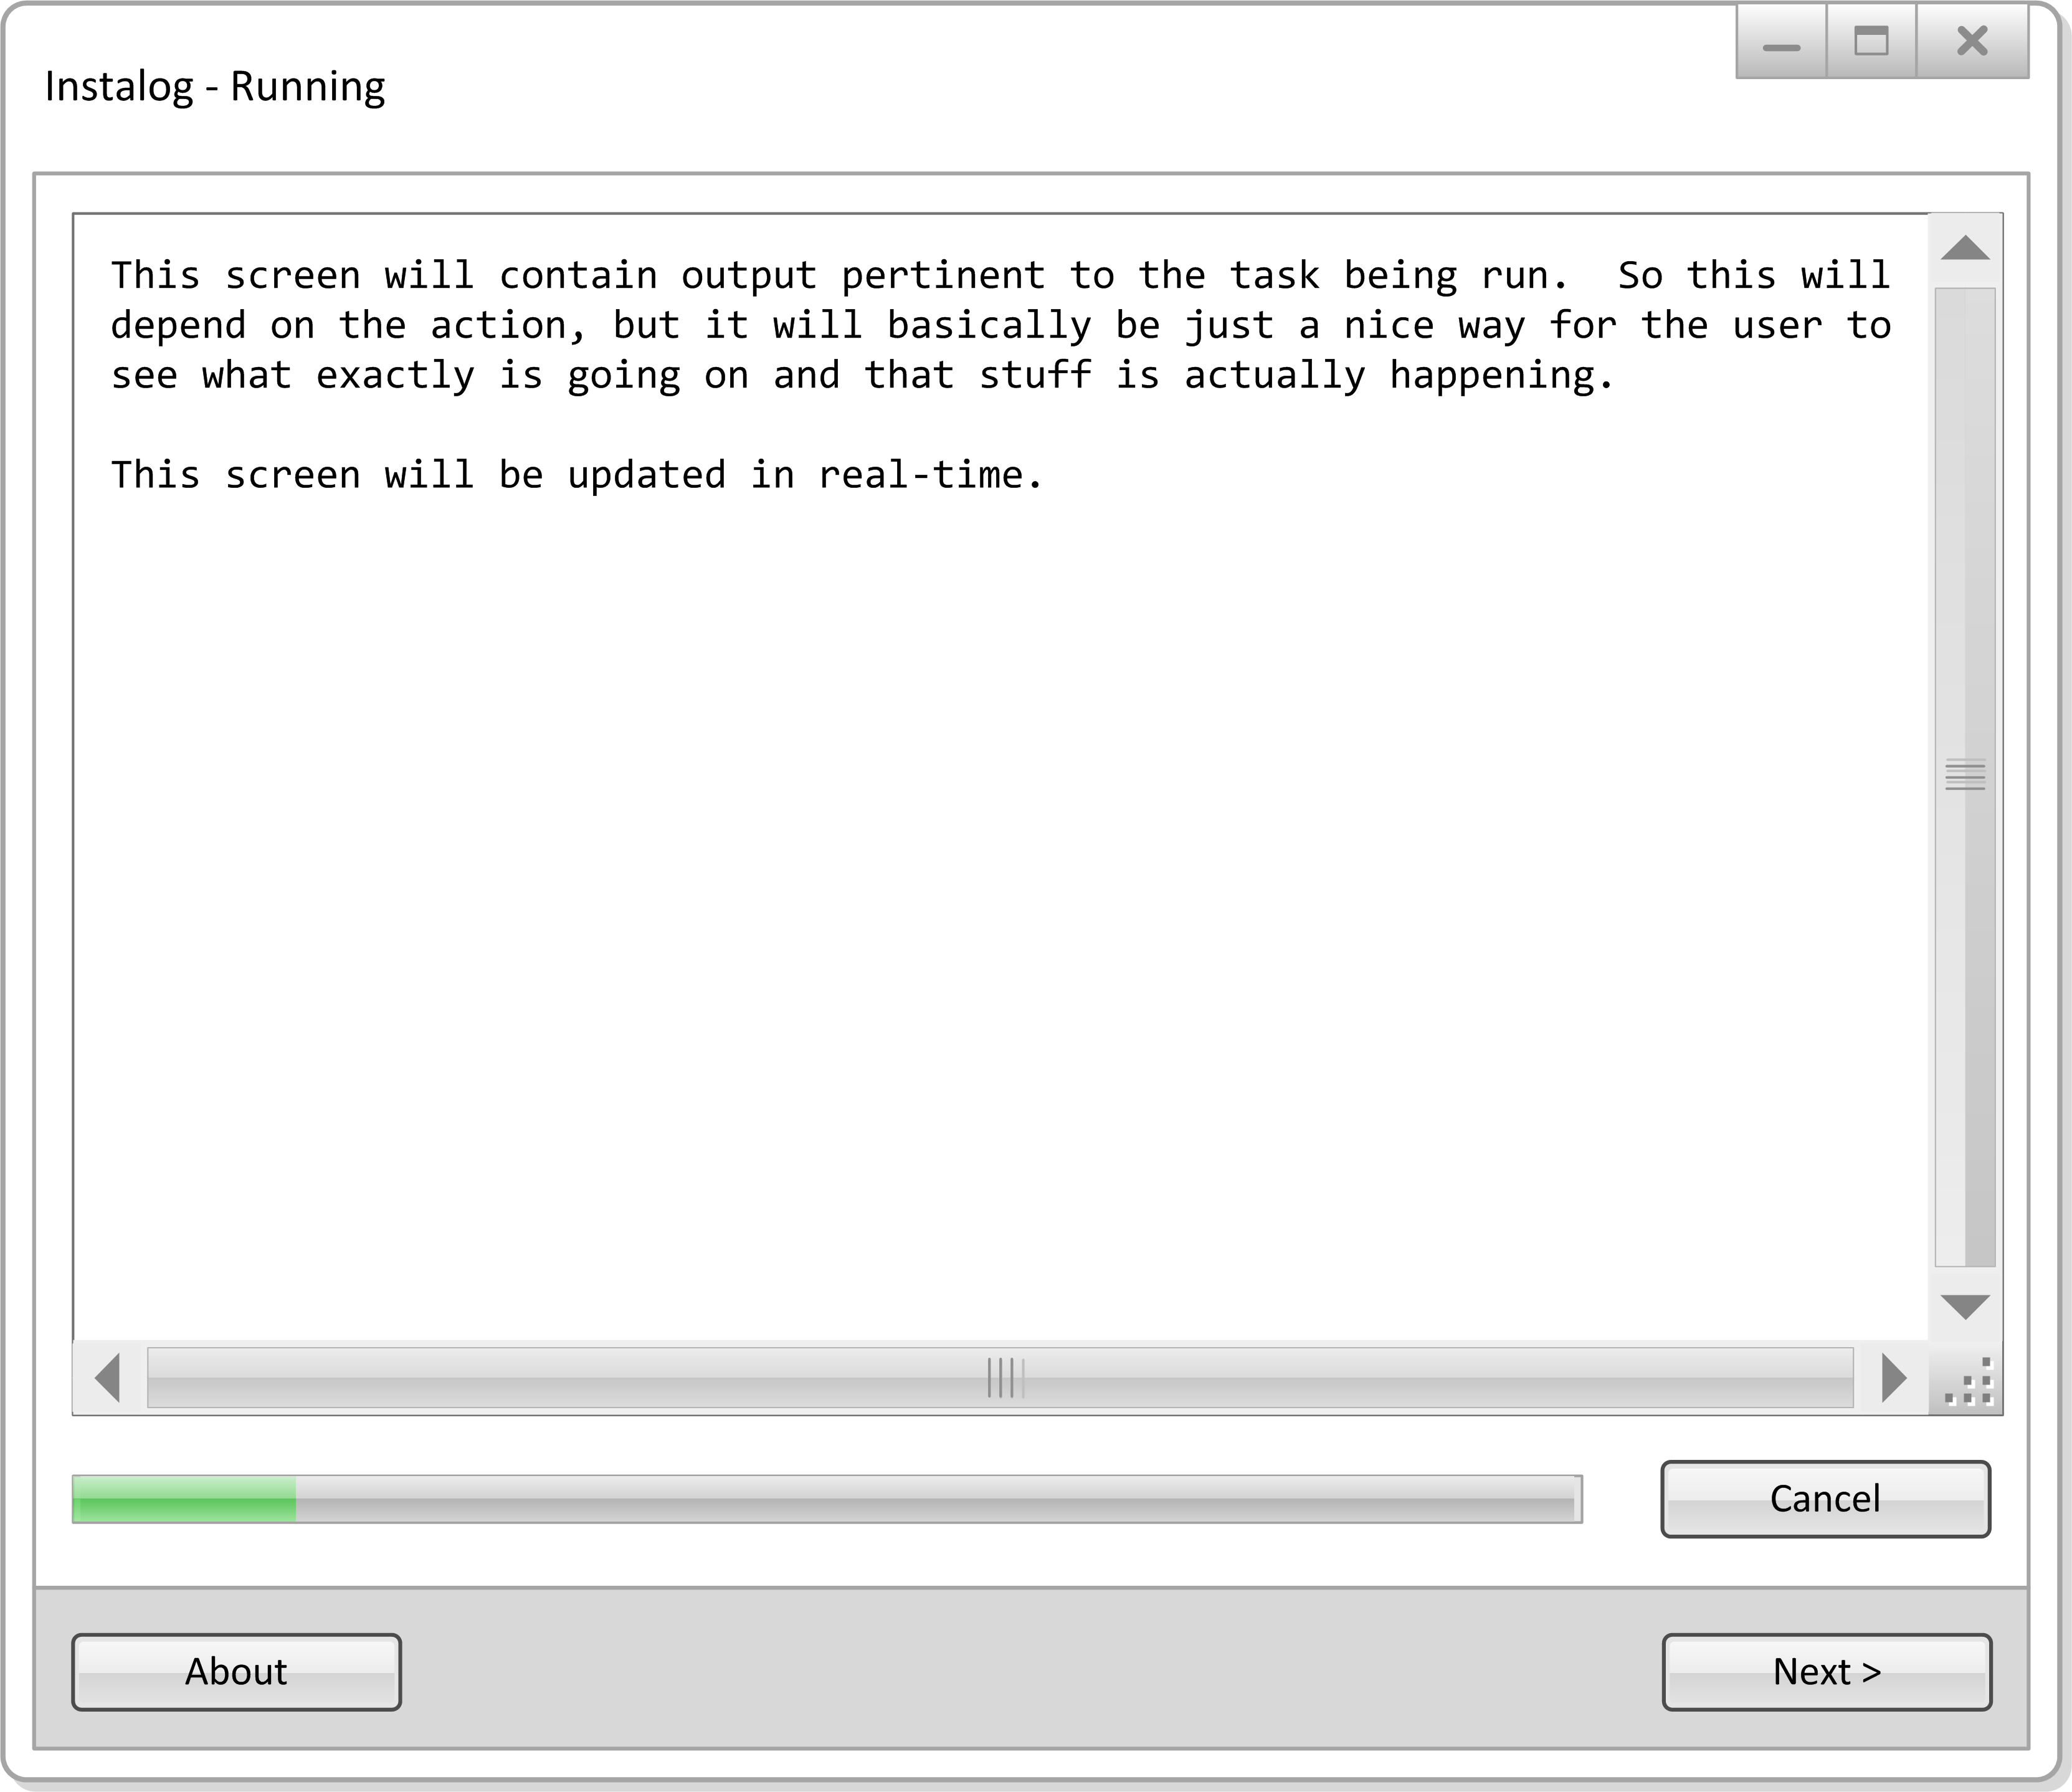
\includegraphics{figures/gui/Running.png}
  	\caption{GUI Running Screen}
  	\label{fig:gui_running}
\end{figure}

\begin{description}
\item[Textbox requirements] \hfill 
\begin{enumerate}
  \item The textbox shall be updated to display the (raw) log output of the
  currently running screen.  This textbox shall only be updated at a rate of 60
  Hz to avoid slowing down the GUI.
  \item The textbox must be scrollable.  It shall automatically scroll down to 
  follow the output by default.  If the user scrolls up for any reason, it shall
  no longer auto-scroll unless the user manually scrolls all the way down to the
  bottom of the output.
\end{enumerate}
\item[Progress bar requirements] \hfill 
\begin{enumerate}
  \item The progress bar shall contain the best estimate of the progress through
  the script.  This estimate can be something as simple as the completed script 
  actions divided by the total script actions.
\end{enumerate}
\item[Cancel button requirements] \hfill 
\begin{enumerate}
  \item The ``Cancel'' button must not be enabled if the script contains any 
  system-altering actions.  This can be determined by scanning the script in 
  advance.
  \item If the user presses the ``Cancel" button, the ``Next" button must  
  change to display ``Exit."  The text of the ``Cancel" button shall change to
  ``Re-run."  The behavior of both of these buttons should be self-explanatory.
  \item When the script completes, if the script was not a system-altering
  script, then the button should change to ``Re-run."  Otherwise, it shall
  remain displaying ``Cancel" and be disabled.
\end{enumerate}
\item[Window close button requirements] \hfill 
\begin{enumerate}
  \item The window close button must not be enabled if the script contains any 
  system-altering actions.  This can be determined by scanning the script in
  advance.
  \item If the user presses the window close button at any time that it is
  enabled, a Yes/No dialog should appear that reminds the user that the script
  output has not been saved yet.
\end{enumerate}
\item[Next button requirements] \hfill 
\begin{enumerate}
  \item The ``Next" button shall not be enabled until after the script 
  completes.
  \item When the user presses the ``Next" button, the tool shall proceed to the
  Run Completed Screen (section~\ref{sec:run_completed_screen}).
\end{enumerate}
\end{description}

\subsection{Run Completed Screen} \label{sec:run_completed_screen}
This screen enables a user to decide what to do with their script output (log
file).  This screen is presented in Figure~\ref{fig:gui_run_complete}.

\begin{figure}[h]
  	\centering
	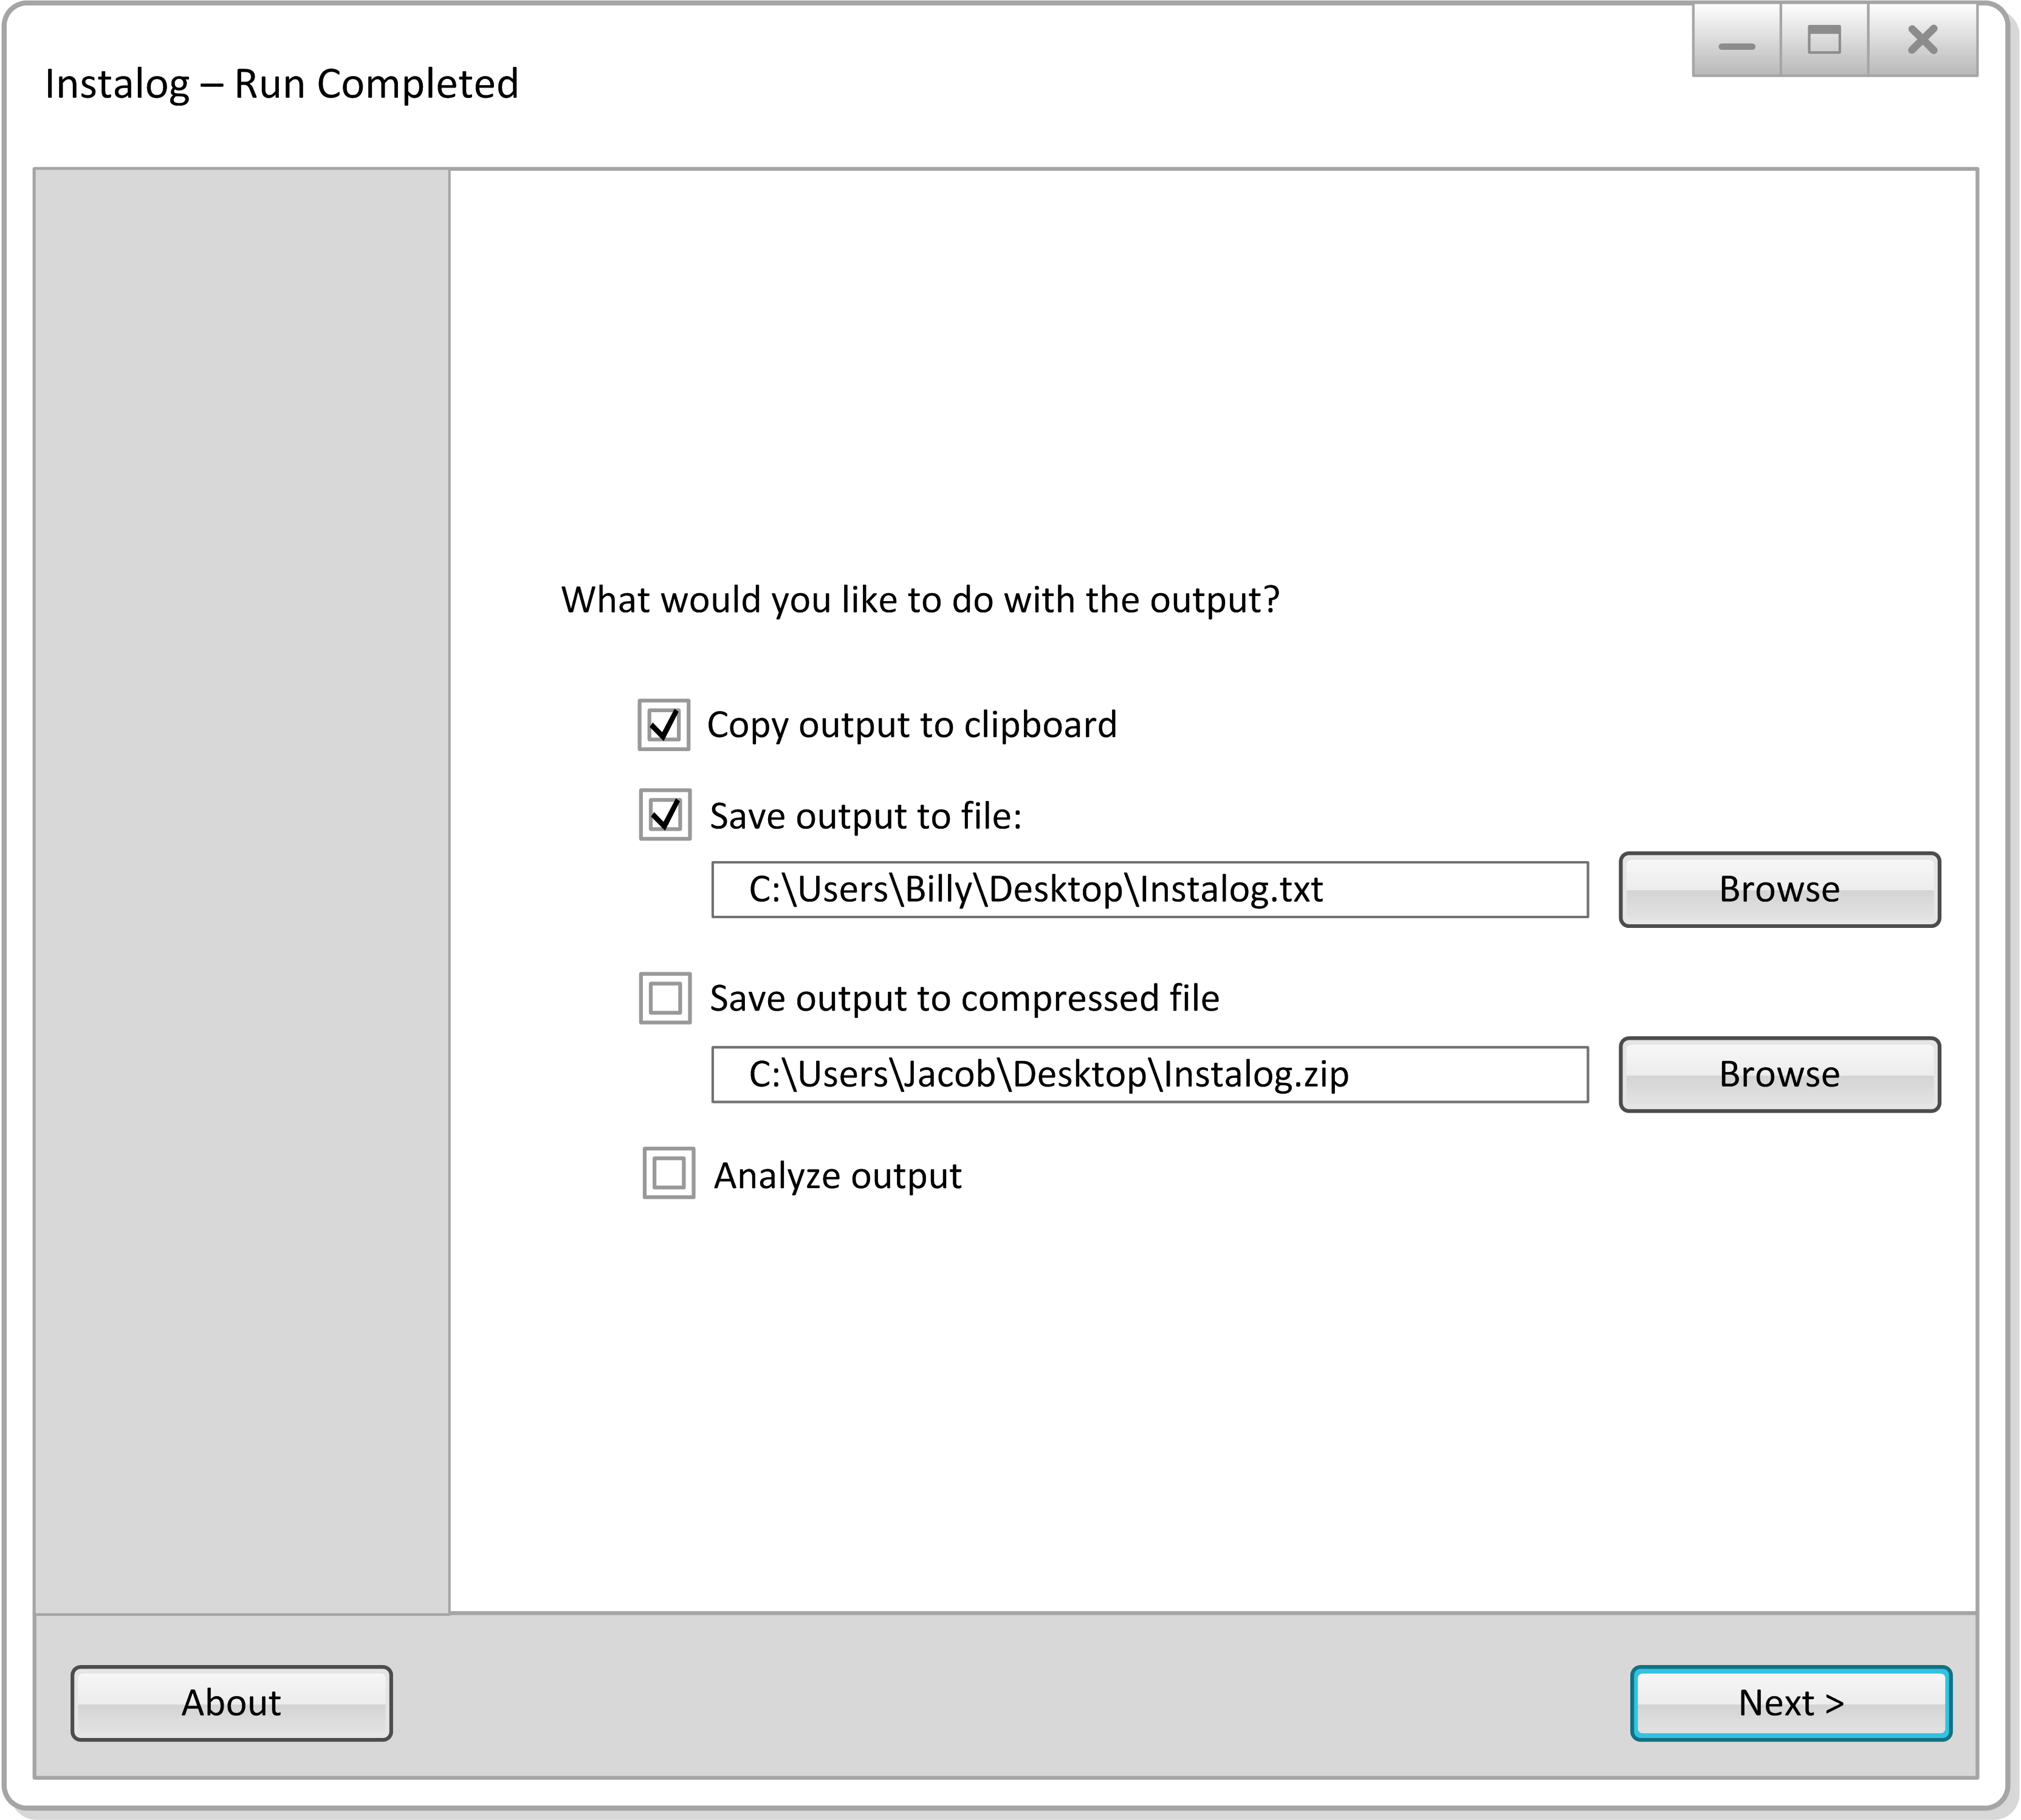
\includegraphics{figures/gui/Run_Completed.png}
  	\caption{GUI Run Complete Screen}
  	\label{fig:gui_run_complete}
\end{figure}

\begin{description}
\item[Option requirements] \hfill
\begin{enumerate}
  \item By default, nothing shall be selected
  \item Both of the file Save fields shall default to the user's desktop
  (\verb|%userprofile%\Desktop\|) with the filenames \verb|Log.txt| and
  \verb|Log.zip|.
\end{enumerate}
\item[Next button requirements] \hfill
\begin{enumerate}
  \item The button must be disabled until at least one option is selected. It
  must return to being disabled if nothing is selected.
  \item The button shall have the following behavior when it is clicked:
  \begin{enumerate}
    \item If the options selected did not include ``Analyze output," then the
    tool shall proceed to the Finished Screen
    (section~\ref{sec:finished_screen}).
    \item If the options selected include ``Analyze output" and other options,
    then the other options shall execute and then the tool should proceed to
    the Analysis Screen (section~\ref{sec:analysis_screen}).
    \item If the only option selected was ``Analyze output," then the tool
    shall proceed to the Analysis Screen (section~\ref{sec:analysis_screen})
    after displaying a warning that the output will be otherwise un-savable.
  \end{enumerate}
\end{enumerate}
\item[Window close button requirements] \hfill
\begin{enumerate}
  \item If the user presses the window close button at any time that it is
  enabled, a Yes/No dialog shall appear that reminds the user that the script
  output has not been saved yet.
\end{enumerate}
\end{description}


\subsection{Analysis Screen} \label{sec:analysis_screen}
The analysis screen enables users to construct a script based on the output
from a log.  For the requirements listed in this section, it does not
matter what workflow the user used to get to this screen.  This screen is
presented in figure~\ref{fig:gui_analyze}.

\begin{figure}[h]
  	\centering
	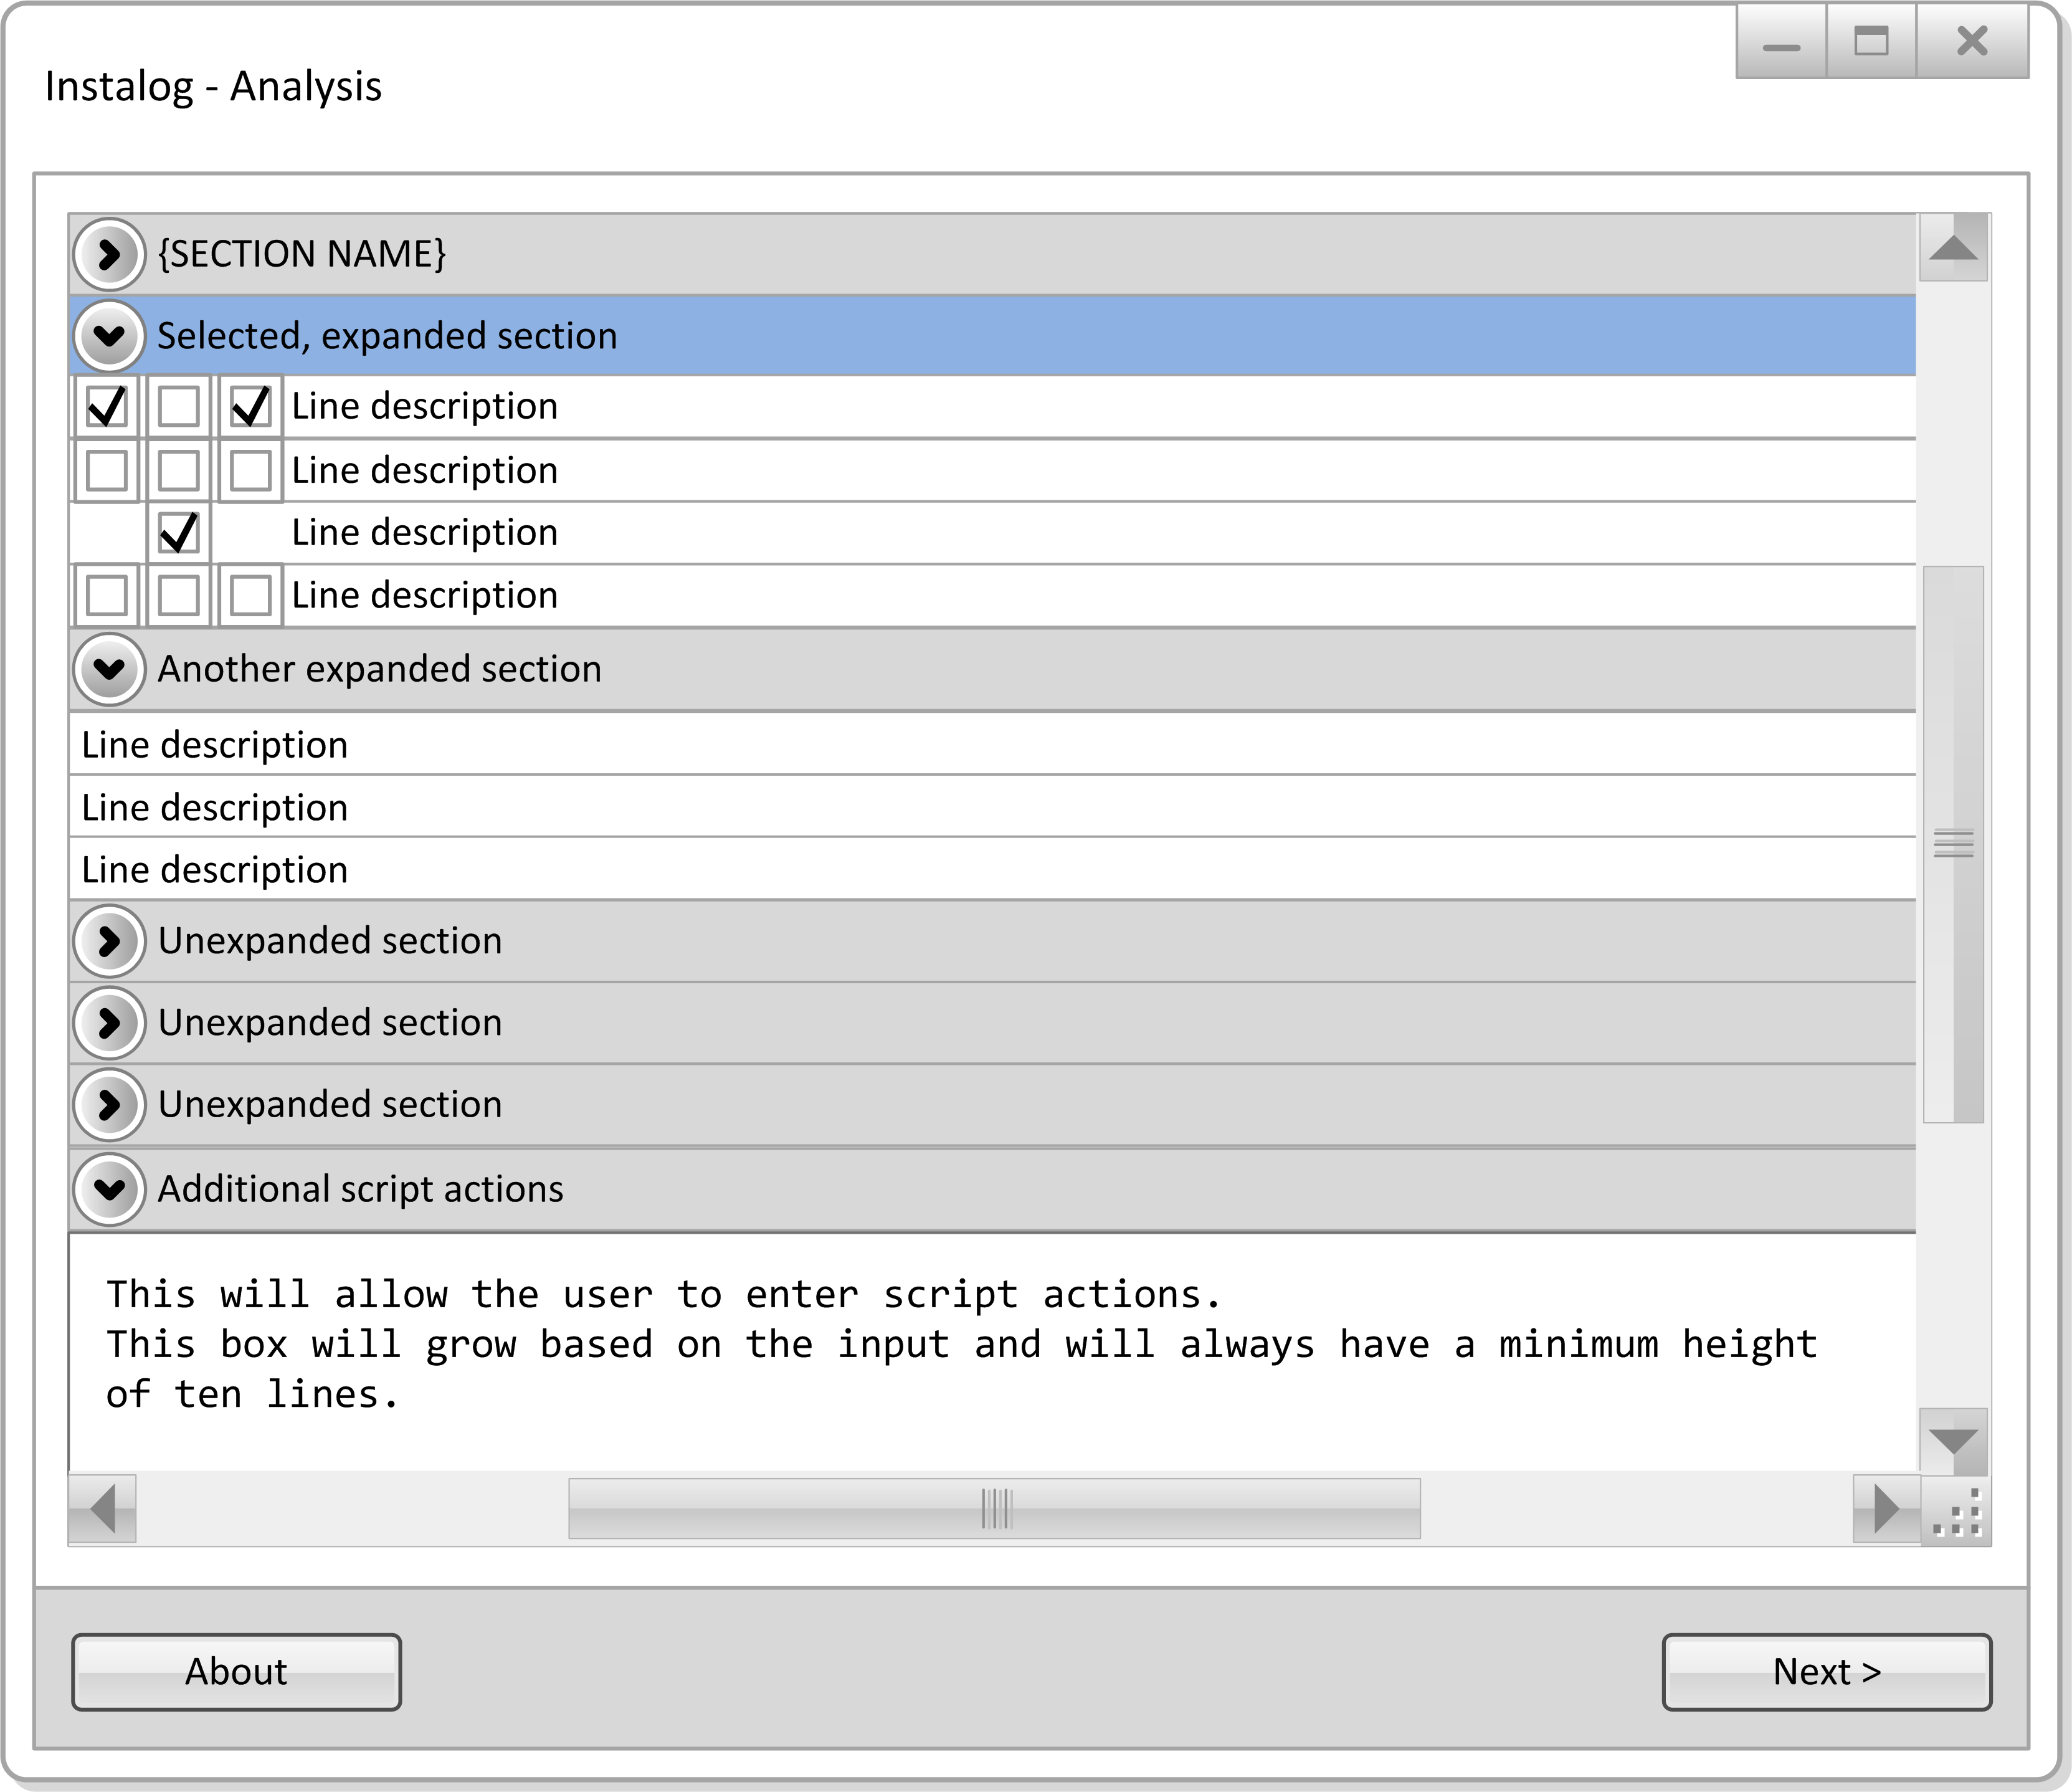
\includegraphics{figures/gui/Analysis.png}
  	\caption{GUI Analysis Screen}
  	\label{fig:gui_analyze}
\end{figure}

\begin{description}
\item[Section heading requirements] \hfill
\begin{enumerate}
  \item Each separate section in the log shall be parsed into one of the gray
  section.  Sections in the log are described in section~\ref{sec:log_output}.
  \item Sections can be collapsed or expanded by the user.  The user can either
  press the entire section heading or the Chevron arrow to perform this action.
  By default, all sections will be expanded.
  \item The Chevron arrow shall point to the right for collapsed sections and
  downward for expanded sections.
  \item No animation is necessary for the collapse action or expand action.
  \item Hovering over a section shall slightly change the background color.
  \item Each corresponding line shall be listed under the section.  Some
  sections might not have any lines.  In this case, a single line shall appear
  with the following text in italics: ``No lines available for this section."
\end{enumerate}
\item[Line requirements] \hfill
\begin{enumerate}
  \item Each separate line of the log will be logged into a line underneath the
  corresponding section.
  \item Hovering over a line shall slightly change the background color.
\end{enumerate}
\item[Checkbox requirements] \hfill
\begin{enumerate}
  \item Depending on the line, there may be zero, one, or many actions available
  for the given line.  There shall be a checkbox to the left of the line for
  each action.  Checking a box indicates that the action shall be taken.
  \item A user shall be able to hover their mouse over any checkbox to
  determine what action the checkbox enables.
  \item In a given section, actions shall be grouped by actions.  Therefore,
  each column will only have one type of action in it.  If an action does not
  apply to a line, there shall simply be an empty slot where the checkbox would
  be.
  \item All checkboxes shall default to unchecked.
\end{enumerate}
\item[Aditional script actions requirements] \hfill
\begin{enumerate}
  \item The last section in the log must always be titled ``Additional script
  actions'' and will contain a textbox that will allow the user to specify
  additional script actions to take
  \item The textbox shall always have a minimum height of ten lines and will
  grow to always be one line longer than its contents
  \item The textbox shall not have its own scrollbars.  Rather, the scrollbars
  for the rest of the control are be sufficient
  \item The textbox must support basic operations including but not limited
  to Copy, Paste, and Undo/Redo.
  \item The textbox shall not implement word-wrap.
\end{enumerate}
\item[Next button requirements] \hfill
\begin{enumerate}
  \item The Next button shall display a Yes/No dialog warning the user that
  scripts are final and there is no going back.
\end{enumerate}
\end{description}

\subsection{Analysis Completed Screen}
This screen enables a user to decide what to do with the finished script.  This
screen is presented in Figure~\ref{fig:gui_analysis_completed}.

\begin{figure}[h]
  	\centering
	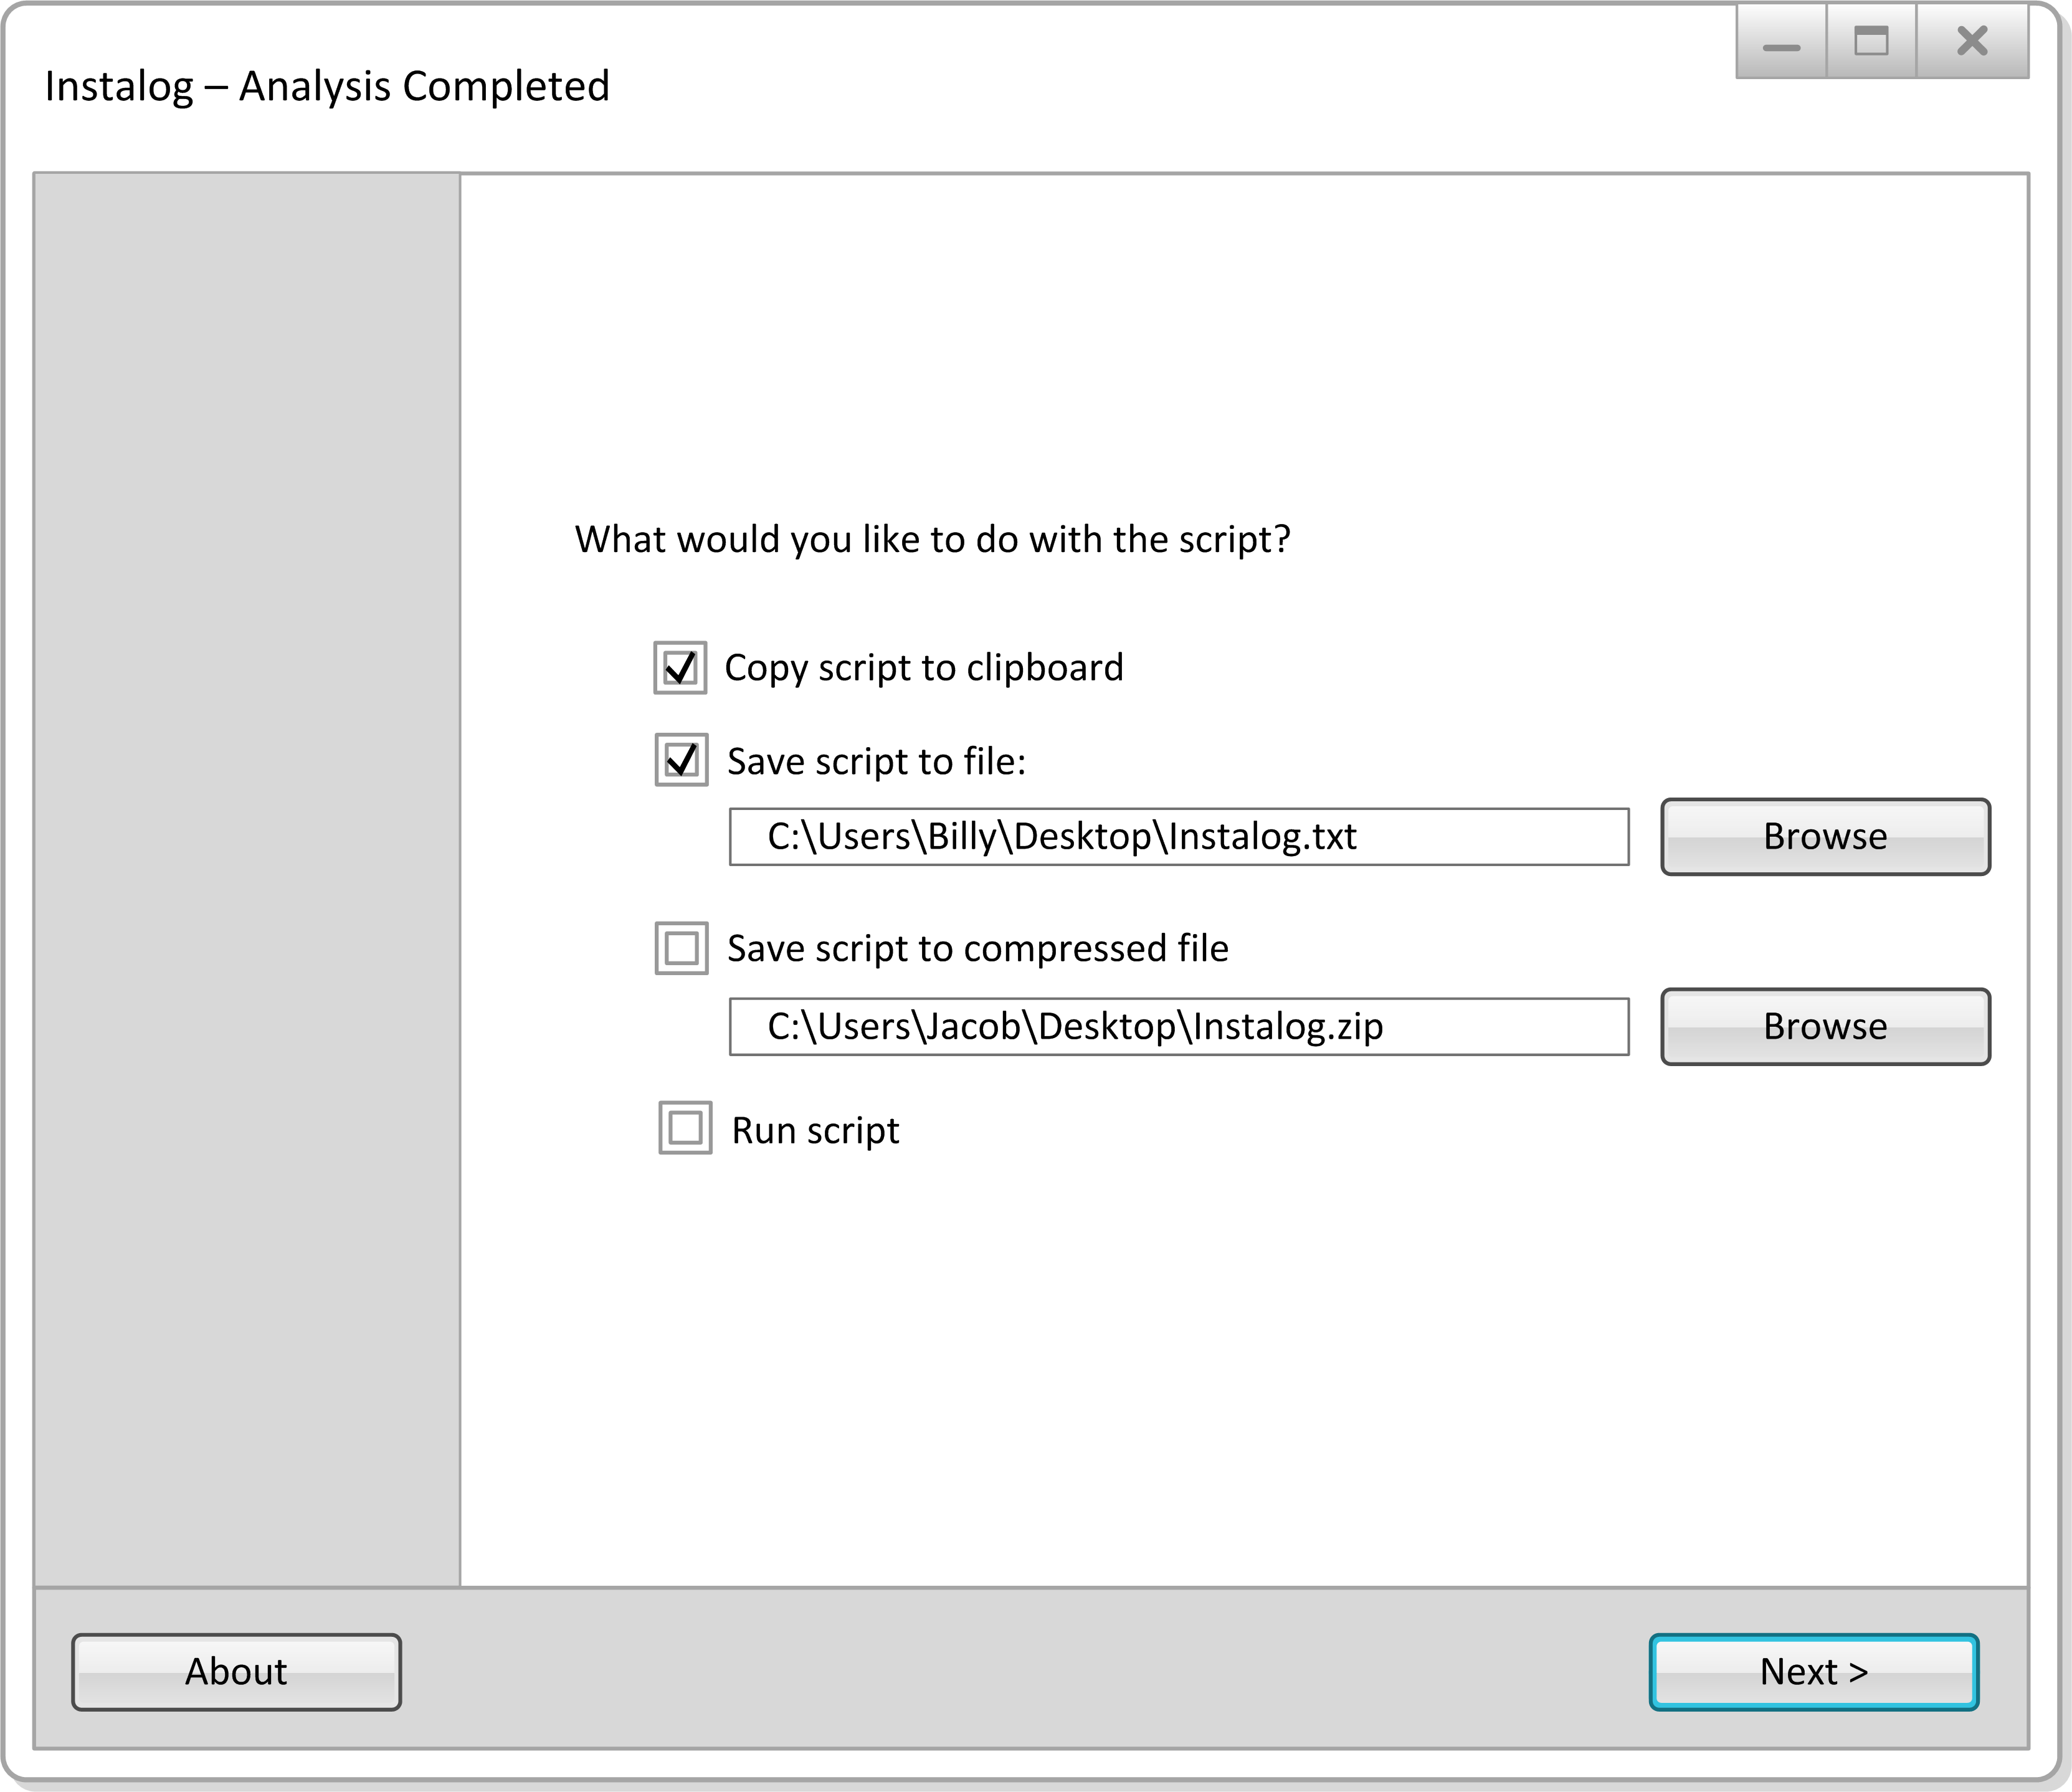
\includegraphics{figures/gui/Analysis_Completed.png}
  	\caption{GUI Analysis Completed Screen}
  	\label{fig:gui_analysis_completed}
\end{figure}

\begin{description}
\item[Option requirements] \hfill
\begin{enumerate}
  \item By default, nothing shall be selected
  \item Both of the file Save fields shall default to the user's desktop
  (\verb|%userprofile%\Desktop\|) with the filenames \verb|Script.txt| and
  \verb|Script.zip|.
\end{enumerate}
\item[Next button requirements] \hfill
\begin{enumerate}
  \item The button must be disabled until at least one option is selected. It
  must return to being disabled if nothing is selected.
  \item The button shall have the following behavior when it is clicked:
  \begin{enumerate}
    \item If the options selected did not include ``Run script," then the tool
    shall proceed to the Finished Screen (section~\ref{sec:finished_screen}).
    \item If the options selected include ``Run script" and other options, then
    the other options shall execute and then the tool shall proceed to the
    Running Screen (section~\ref{sec:running_screen}).
    \item If the only option selected was ``Run script," then the tool shall
    proceed to the Running Screen (section~\ref{sec:running_screen}).
  \end{enumerate}
\end{enumerate}
\item[Window close button requirements] \hfill
\begin{enumerate}
  \item If the user presses the window close button at any time that it is
  enabled, a Yes/No dialog must appear that reminds the user that the script
  has not been saved yet.
\end{enumerate}
\end{description}

\subsection{Finished Screen} \label{sec:finished_screen}
The finished screen provides the user with some confirmation that the actions
instructed of the tool were actually executed.  This is to prevent users from
becoming disoriented and thinking that the tool had crashed or something else
bad had happened.  This screen is presented in Figure~\ref{fig:gui_finished}.

\begin{figure}[h]
  	\centering
	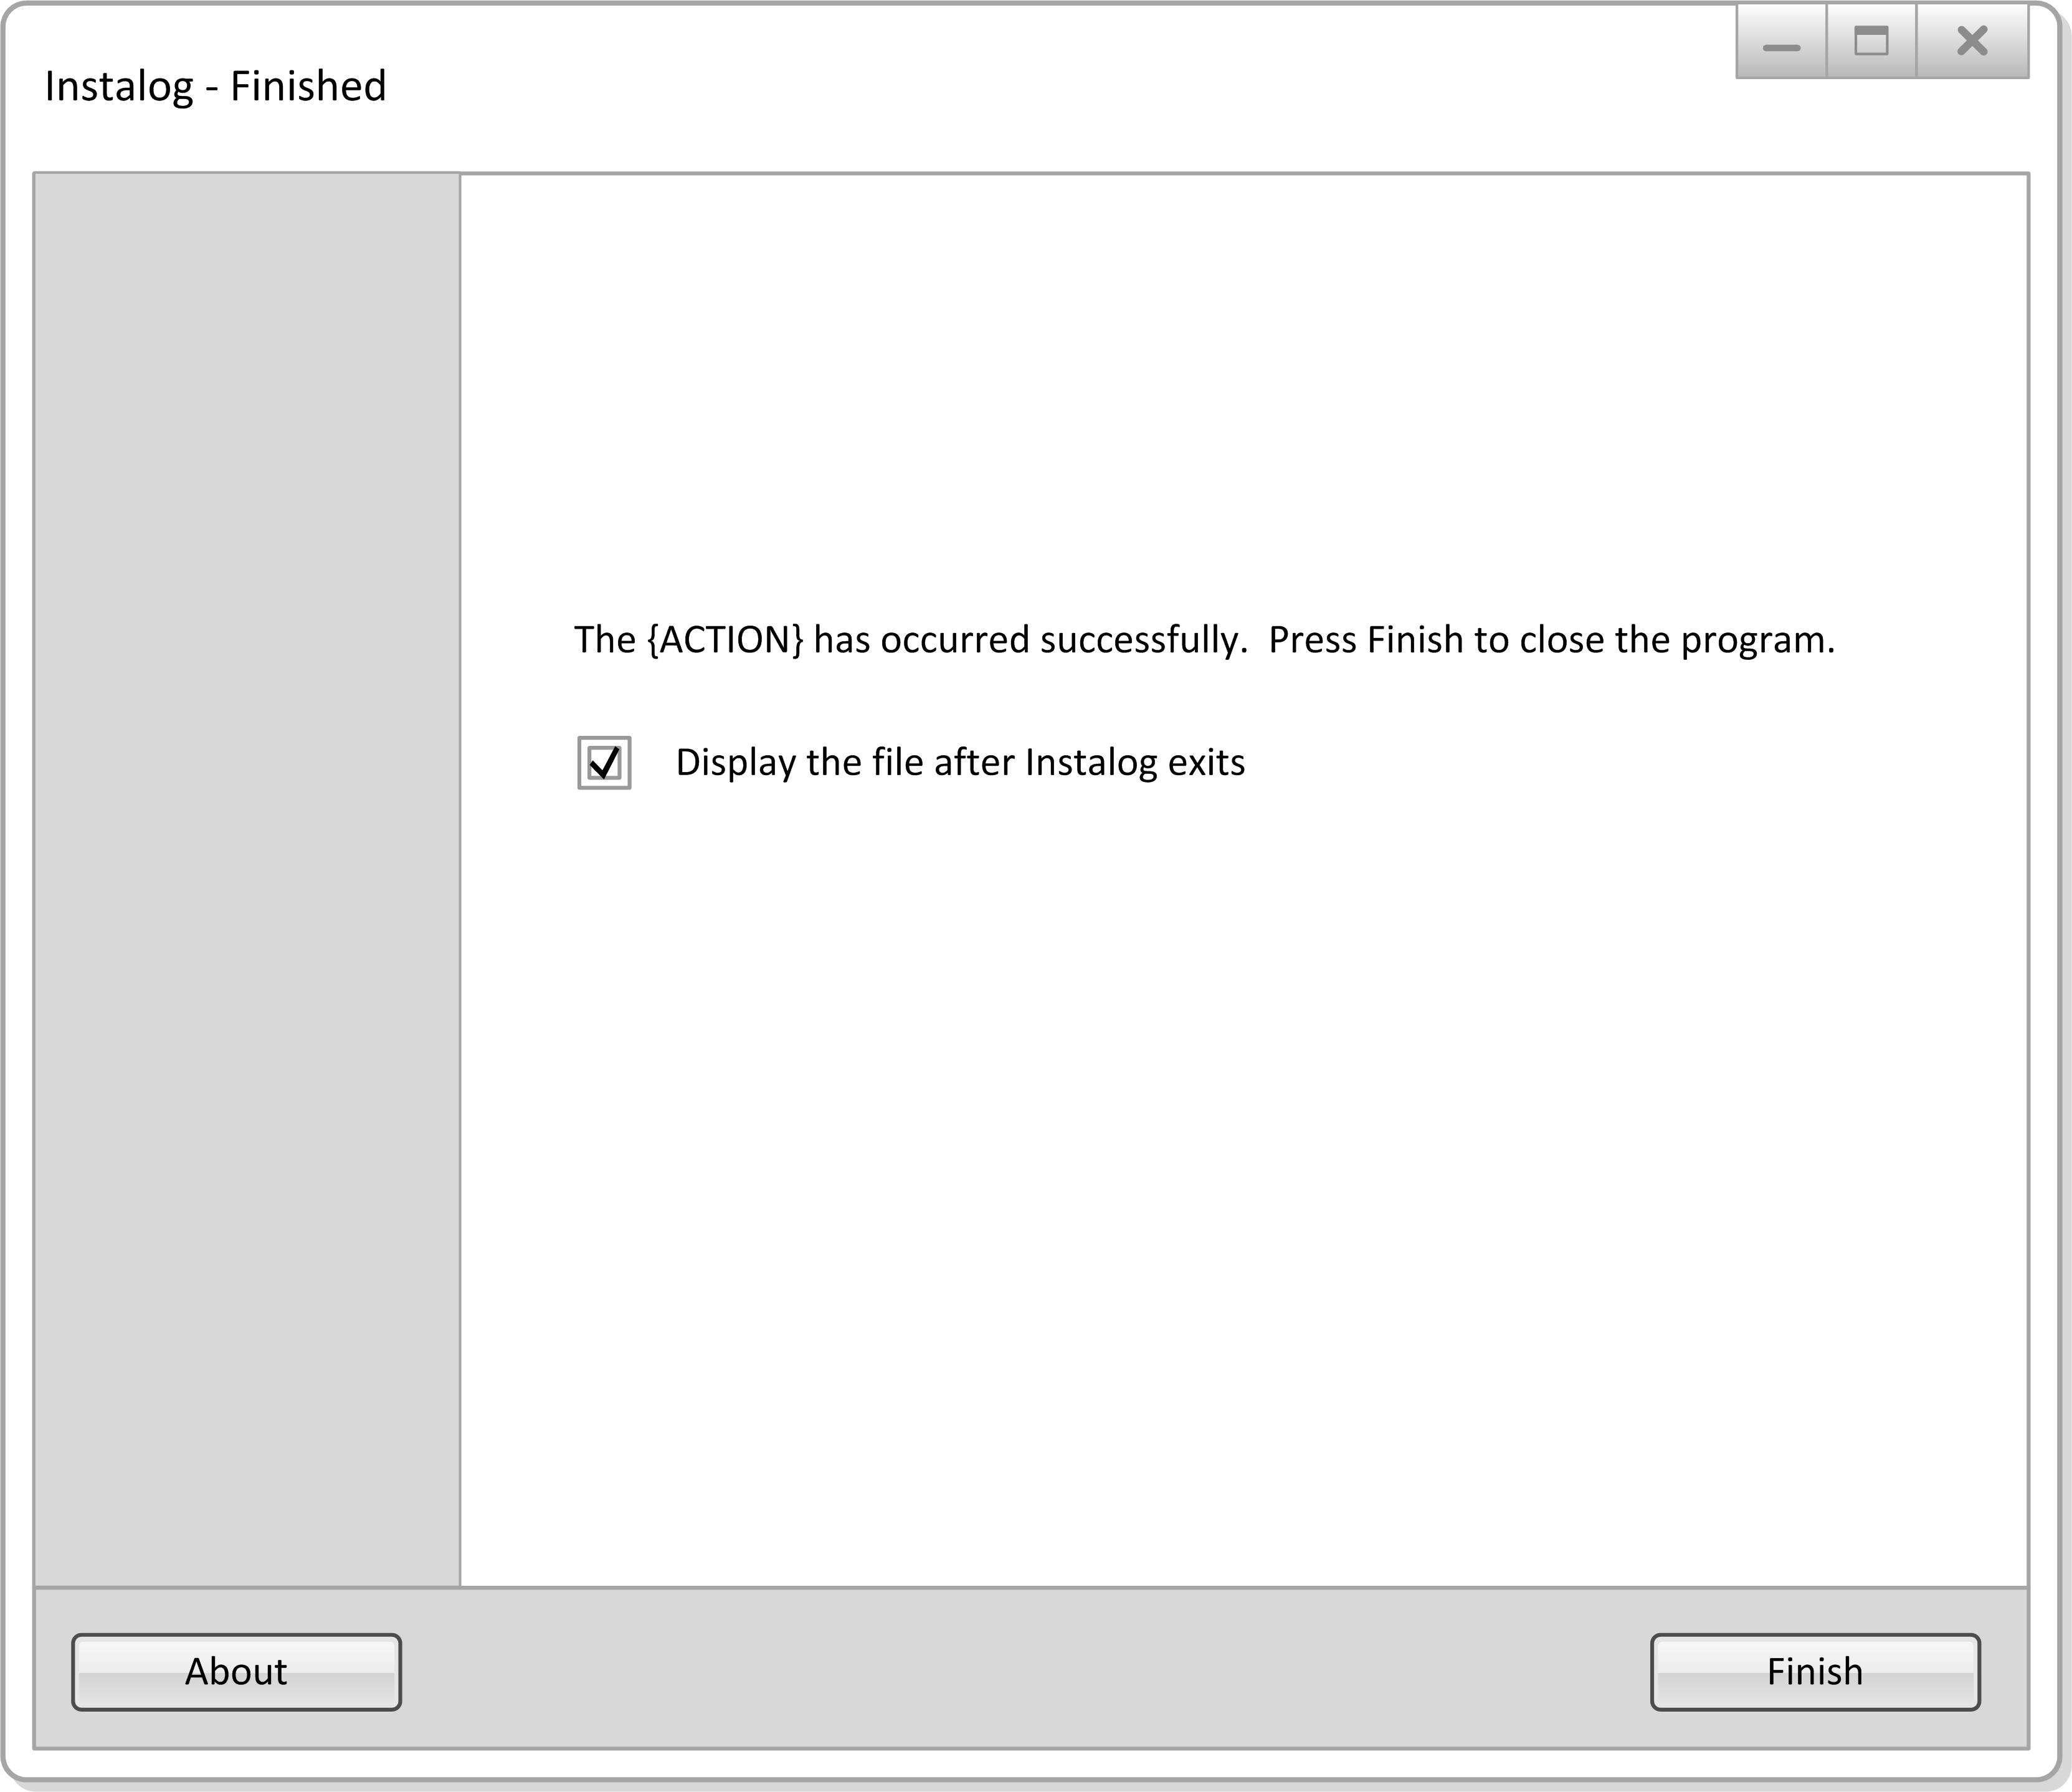
\includegraphics{figures/gui/Finished.png}
  	\caption{GUI Finished Screen}
  	\label{fig:gui_finished}
\end{figure}

\begin{description}
\item[Text requirements] \hfill
\begin{enumerate}
  \item The text shall display some information about what happened.  The text
  should cover all possible combinations of copying material to the clipboard,
  saving one file, or saving two files.
\end{enumerate}
\item[Display file checkbox requirements] \hfill
\begin{enumerate}
  \item If a plaintext file was saved, then a checkbox shall be displayed that
  allows the user to specify if they want to view the file when the program
  exits.
  \item The default state of this checkbox shall be unchecked.
  \item Upon exiting, if this is checked, notepad shall be launched and display
  this file.
\end{enumerate}
\end{description}

\subsection{Flowchart}
Since there are several different branch points in the tool, the flow through
the tool is difficult to describe by simply using text.  The flow described in
the preceding sections is described in Figure~\ref{fig:gui_flowchart} in
flowchart form.

\begin{figure}[h!]
  	\centering
	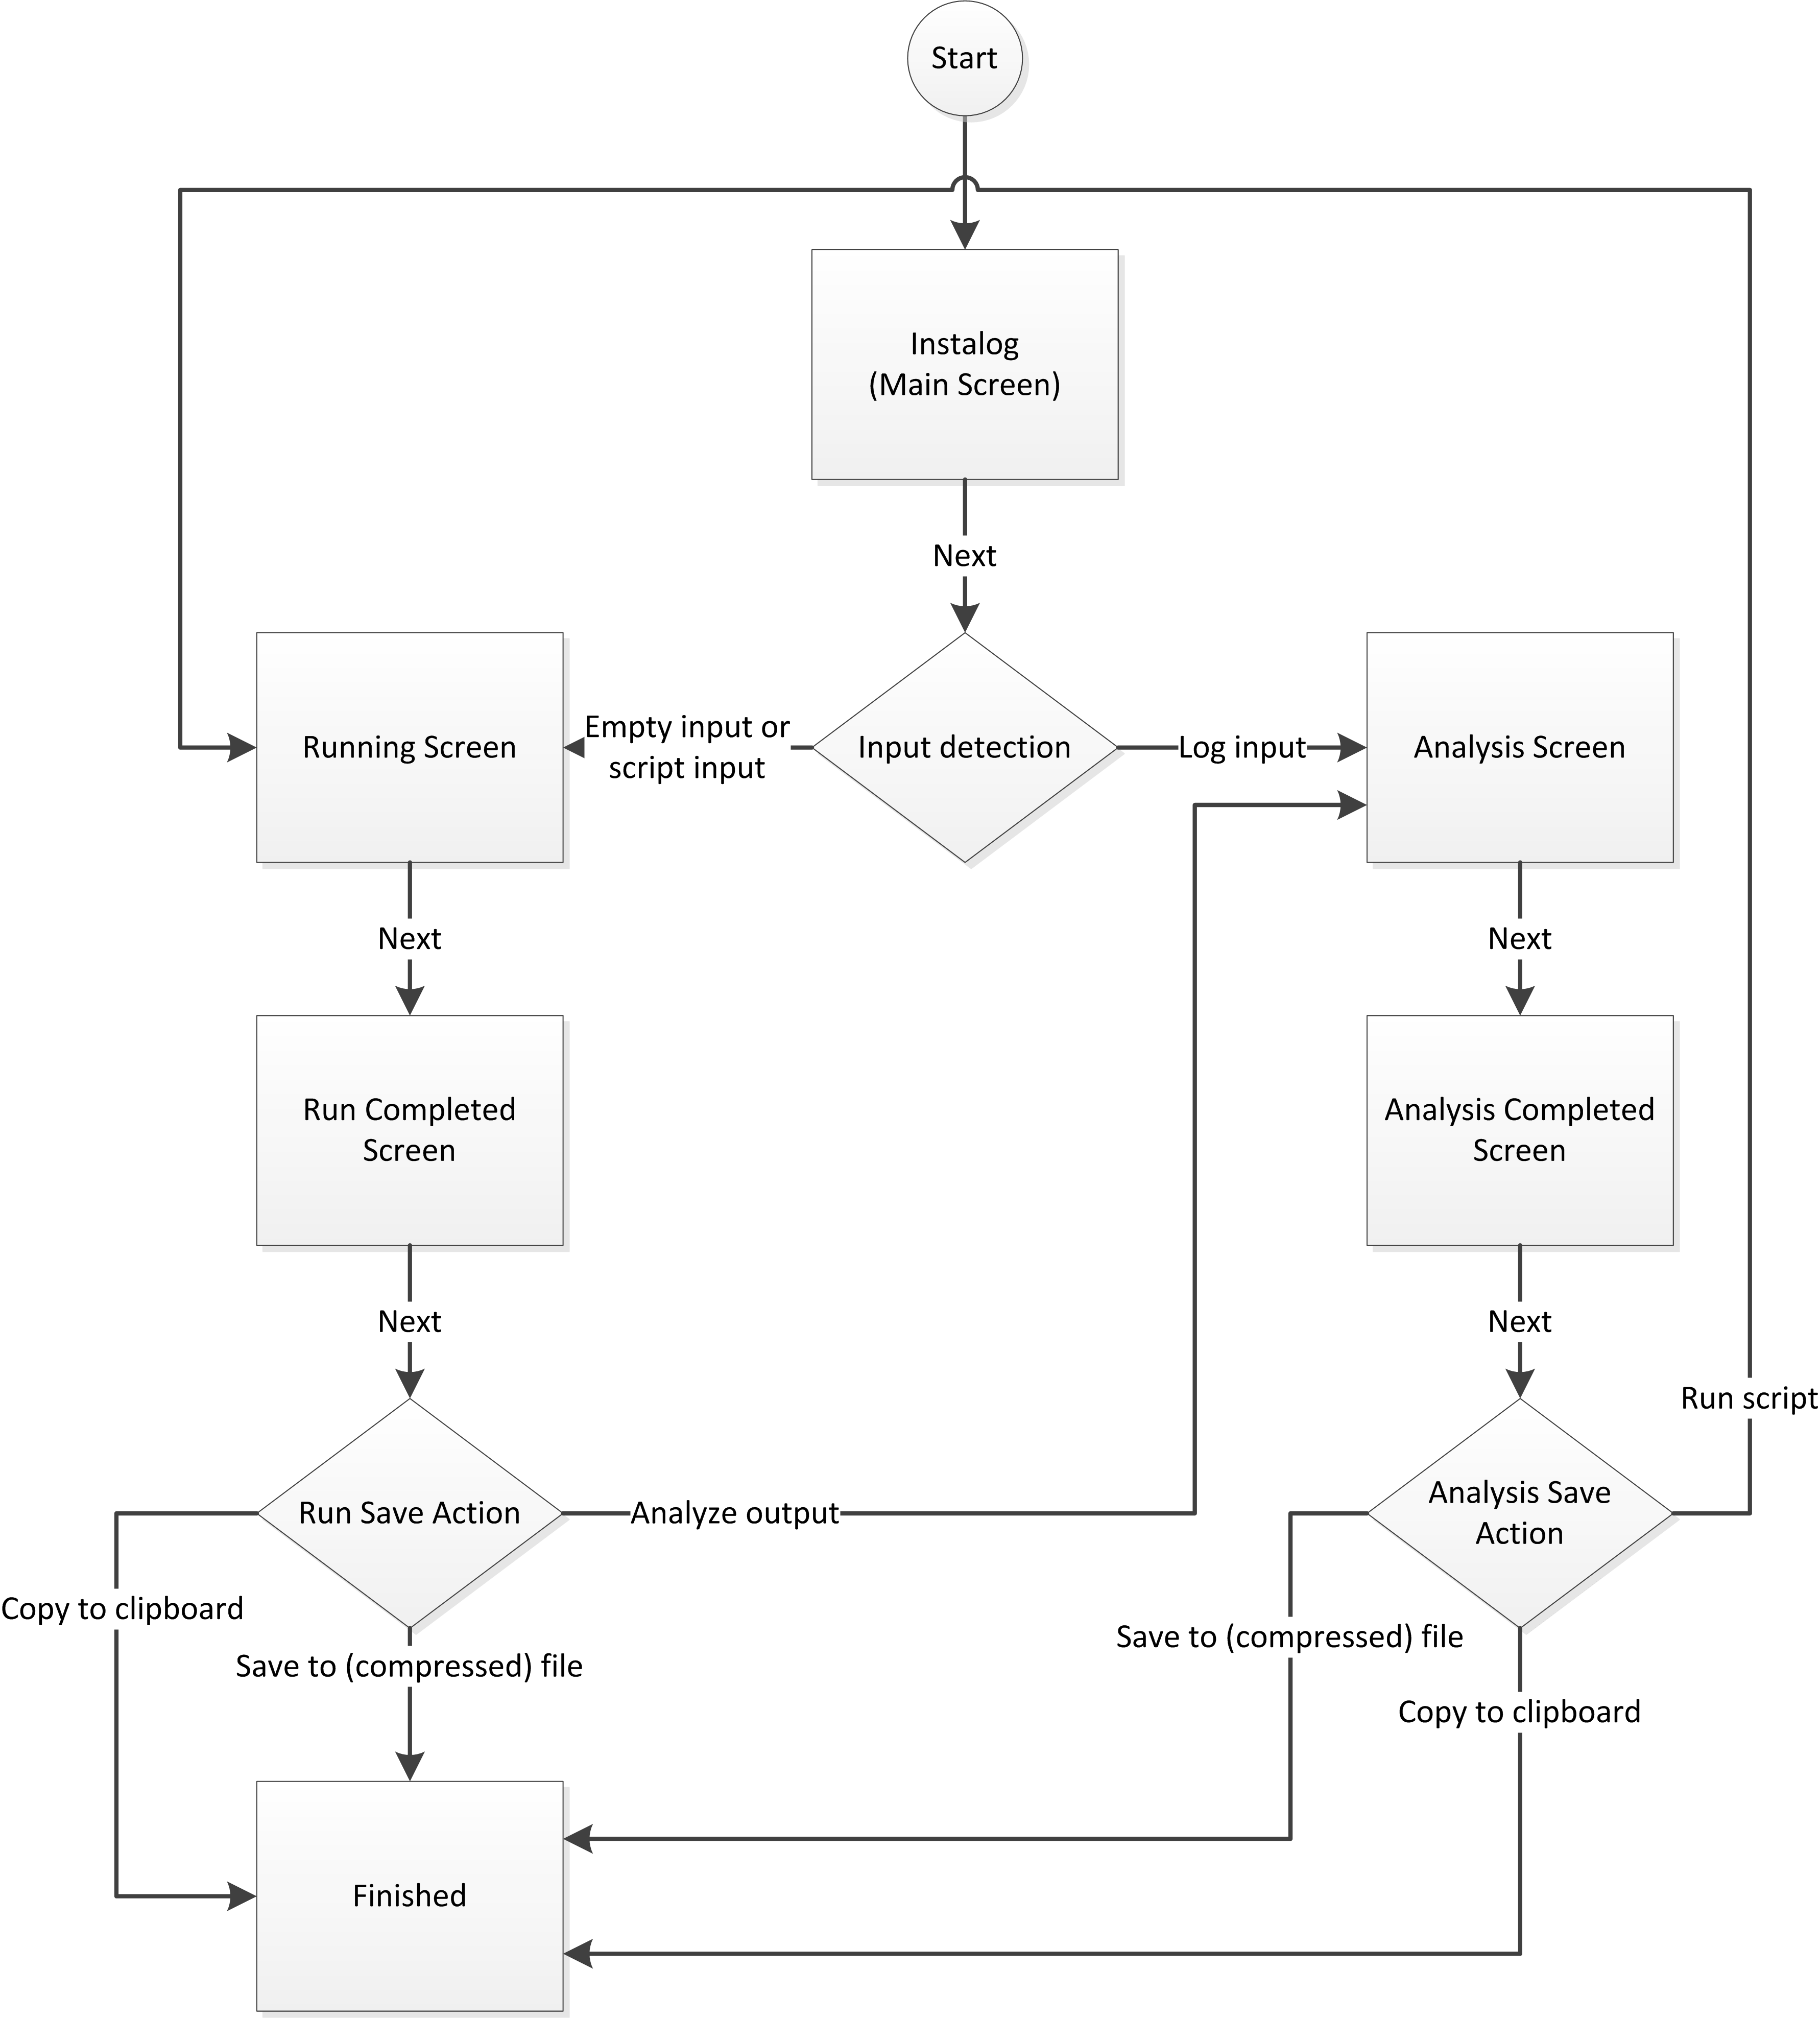
\includegraphics{figures/gui/GUI_Flowchart.png}
  	\caption{GUI Flowchart}
  	\label{fig:gui_flowchart}
\end{figure}

Portions of this document are written in terms of the \verb|.REG| format
described by Regedit, a Widnows component. The syntax for the regedit script is
described in several locations, in particular  of \texttt{monospaced}
(\url{http://en.wikipedia.org/wiki/Windows_Registry#.REG_files}).

Additionally WOW64 (Windows on Windows 64) defines a system whereby registry
virtualization is in effect -- 32 bit programs are shown a virtualized view of
the 64 bit registry. Current versions of windows implement this by putting the
32 bit registry view in a key called ``\verb|Wow6432Node|'' in the root of each
hive in the registry. Additionally, Windows provides flags to the functions that open
registry keys, such as \verb|NtOpenKey| or \verb|RegCreateKeyEx|, which select
the correct view. Microsoft asks that applications be built in terms of the API
flags, because the specific name of \verb|Wow6432Node| is an implementation
detail which can change in future versions of Windows.

Therefore, we will define on top of the \verb|.REG| format a comment of
\verb|;32 Bit Registry View| or \verb|64 Bit Registry View|, which represent the
flag that would be passed into Windows when opening the indicated key.

\section{Log Output} \label{sec:log_output}
This section generally defines the form of Instalog's output. A log is split up
into several delimited portions called ``sections''. With the exception of
headers and footers, all sections begin with a line of the following format:

\begin{verbatim}
================ ${Section Name} ===============
\end{verbatim}

That is, the name of the section with one space of padding, centered in a block
of equals (\verb|=|) signs 50 total characters wide. In the case that a tie
exists with respect to the centering, Instalog shall prefer placing the name of
the section farther to the right than to the left.

\subsection{Default Script Sections} \label{sec:default_script_sections}
Instalog's standard (that is, run without a script) output consists of the
following sections in the following order:
\begin{enumerate}
    \item Header
    \item Running Processes
    \item Machine PsuedoHJT Report
    \item $n$ User PseudoHJT Reports (One for each loaded user registry on the
    system)
    \item Mozilla Firefox (If Mozilla Firefox is installed)
    \item Google Chrome (If Google Chrome is installed)
    \item Created Last 30
    \item Find3M Report
    \item Event Viewer (If any relevant events need be reported)
    \item Machine Specifications
    \item Restore Points
    \item Installed Programs
    \item Footer
\end{enumerate}

\subsection{Additional Script Sections}
\noindent{}The following additional sections are available but they are not
generated in the default report:
\begin{description}
\item[DNS Check] Displayed if the \verb|:dnscheck| scripting section is used.
\item[Directory] Displayed if the \verb|:dirlook| scripting section is used.
\item[VirusTotal] Displayed if the \verb|:virustotal| scripting section is used.
\item[MRC Upload] Displayed if the \verb|:mrc| scripting section is used.
\item[Process Kill] Displayed if the \verb|:kill| scripting section is used.
\item[File Quarantine] Displayed if the \verb|:move| scripting section is used.
\item[Security Center] Displayed if the \verb|:securitycenter| scripting section
is used.
\item[Registry 32 Bit] Displayed if the \verb|:reg32| scripting action is used.
\item[Registry 64 Bit] Displayed if the \verb|:reg64| scripting action is used.
\end{description}

\subsection{Escaping Formats}
In order to meet the requirements of machine readability and human readability,
several escaping formats must be used depending on the type of data to produce
the most readable unambiguous representation given typical data collected from a
given location.

\subsubsection{General Escaping Format}
Generally, escaping MUST be done in a manner similar to most programming
languages, such as C, C++, Java, or similar, for quoted string escapes. Such an
escaping scheme is defined by three characters: an optional starting delimiter,
an optional termination delimiter, and an escape character. For instance, in C,
the starting delimiter is the quote mark, \verb|"|, the ending delimiter is also
a quote mark \verb|"|, and the escape character is the backslash \verb|\|.

For most types of information Instalog enumerates, such as Windows file paths,
the exact method C uses is unsuitable; backslashes occur far too often inside
file paths for the backslash as an escape character to make a good choice.
Legacy applications like the command processor (\texttt{cmd.exe}) get around
such problems by implementing complicated escaping schemes, but these are
designed with specific input data in mind (file paths and command line
switches, for instance), which is not the case for most reported data.

\label{generalescape}
Therefore, Instalog shall use define a general escape function that works in a
manner similar to C's string literal escapes, but which allows arbitrary
starting, termination, and escaping characters. The input to the escape function
is raw data obtained from some data source, and the output is the same data with
the following textual replacements: 

\begin{itemize}
    \item \var{EscapeCharacter} is replaced with
    \var{EscapeCharacter}\var{EscapeCharacter}.
    \item \var{RightDelimiter}, if defined,  is replaced with
    \var{EscapeCharacter}\var{RightDelimiter}.
    \item The null character (ASCII \verb|0x00|) is replaced with
    \var{EscapeCharacter}\texttt{0}.
    \item The backspace character (ASCII \verb|0x08|) is replaced with
    \var{EscapeCharacter}\texttt{b}.
    \item The form feed character (ASCII \verb|0x0C|) is replaced with
    \var{EscapeCharacter}\texttt{f}.
    \item The newline character (ASCII \verb|0x0A|) is replaced with
    \var{EscapeCharacter}\texttt{n}.
    \item The carriage return character (ASCII \verb|0x0D|) is replaced with
    \var{EscapeCharacter}\texttt{r}.
    \item The horizontal tab character (ASCII \verb|0x09|) is replaced with
    \var{EscapeCharacter}\texttt{t}.
    \item The vertical tab character (ASCII \verb|0x0B|) is replaced with
    \var{EscapeCharacter}\texttt{v}.
    \item ASCII characters which are not in the above list but are unprintable
    (that is, ASCII \verb|0x00| - \verb|0x1F|; \verb|0x7F|) are
    replaced with \var{EscapeCharacter}\texttt{xHH}, where \texttt{HH} is the
    hexadecimal representation of the numeric value of the given character.
    \item Non-ASCII characters (\verb|U+0080| and above) are replaced with
    \var{EscapeCharacter}\texttt{uHHHH}, where \texttt{HHHH} is the hexadecimal
    representation of the numeric value of the character.
    \item Unicode characters requiring a surrogate pair in UTF-16 (that is,
    greater than U+FFFF) are represented as two normal Unicode
    (\var{EscapeCharacter}\texttt{uHHHH}) escapes matching the UTF-16 surrogate
    pair. (This is exactly how they'd be represented in Windows itself.)
    \item Forum software destroys significant whitespace; but escaping every
    space would be impractical. Where there is more than a single consecutive
    space, the second and later spaces are escaped. (That is, replaced with
    ``\var{EscapeCharacter}\texttt{ }''.)
    \item Any instance of \var{EscapeCharacter} followed by an unused character
    in the above list is equivalent to that character with no escape. This will
    never be generated by the escaping functionality in Instalog for general
    escaping, but is valid for the reverse, unescaping, operation.
\end{itemize}

\subsubsection{URL Escaping Format} \label{urlescape}
URL escaping matches the general escaping format above, except has the
additional constraint of forum software which tries to convert URLs into links.
It is desirable to inhibit this behavior of the forum software, so that board
owners need not worry about linking to malicious websites. Therefore, URL
escaping is defined to be general escaping with the additional requirement that
when the string ``\texttt{http}'' (case insensitive) appears, it is replaced
with ``\texttt{htt}\var{EscapeCharacter}\texttt{p}''. This inhibits forum
software's URL behavior which looks for the protocol prefix in order to
determine what portions of a post indicate a link. (Note that due to the last
requirement of general escaping this will cause no effect on the unescaped
data).

\subsubsection{CommandLineToArgvW Escaping Format} \label{winescape}
Windows' own \verb|CommandLineToArgvW| function defines it's own escaping
scheme. This format is delimited on both the left and right by quote (\verb|"|)
characters. Instalog shall interpret this format exactly as Windows' function
does. Quoting MSDN:

\begin{quote}
\verb|CommandLineToArgvW| has a special interpretation of backslash characters
when they are followed by a quotation mark character (\verb|"|), as follows:
\begin{itemize}
    \item $2n$ backslashes followed by a quotation mark produce $n$ backslashes
    followed by a quotation mark.
    \item $(2n) + 1$ backslashes followed by a quotation mark again produce $n$
    backslashes followed by a quotation mark.
    \item $n$ backslashes not followed by a quotation mark simply produce $n$
    backslashes.
\end{itemize}
\end{quote}

\subsection{Date Formats}
Instalog shall use two date formats.

\subsubsection{Standard Date Format} \label{stddate}
The standard date format shall be defined as
\begin{verbatim}
${YYYY}-${MM}-${DD} ${HH}:${MM}:${SS}
\end{verbatim}
Where \var{YYYY} is the four digit year, \var{MM} is the two digit month,
\var{DD} is the two digit day, \var{HH} is the two digit hour, \var{MM} is the
two digit minute count, and \var{SS} is the two digit number of seconds.

If the given value is fewer than the number of digits available, they shall be
zero padded to take up as many spaces as that item has been assigned.

\subsubsection{Millisecond Date Format} \label{millidate}
The millisecond date format shall be defined as
\begin{verbatim}
${YYYY}-${MM}-${DD} ${HH}:${MM}:${SS}.${Milli}
\end{verbatim}
Where \var{YYYY} is the four digit year, \var{MM} is the two digit month,
\var{DD} is the two digit day, \var{HH} is the two digit hour, \var{MM} is the
two digit minute count, \var{SS} is the two digit number of seconds, and
\var{Milli} is the 4 digit number of milliseconds.

If the given value is fewer than the number of digits available, they shall be
zero padded to take up as many spaces as that item has been assigned.

\subsection{Path Formats}
Instalog uses several path formats across it's log output.

\subsubsection{Path Resolution} \label{pathresolution}
Windows often does not provide Instalog with direct path information; providing
a full command line including arguments in some cases. Disambiguating which part
of a given command line is a path to an executable and which is part of the
arguments requires access to the filesystem of the target machine to determine.
Additionally, several APIs used by Instalog return native (NT) paths rather than
Win32 paths as a user would expect. To combat these problems, Instalog must
implement a path resolution facility.

Path resolution consists of three phases:
\begin{enumerate}
    \item Conversion from Native Path to Win32 Path
    \item Separation of the Win32 path from its arguments
    \item Removal of common path prefixes that serve as redirectors
\end{enumerate}

Instalog will use a heuristic to convert from the NT path to the Win32 path; as
there is no consistent API exposed by Windows for this task. This heuristic
consists of replacing several prefixes on the path with known values. These
replacements must be done in the following order.
\begin{enumerate}
    \item If the path begins with \verb|\|, the \verb|\| is removed.
    \item Afterwards, if the path begins with \verb|??\|, the \verb|??\| is
    removed.
    \item Afterwards, if the path begins with \verb|\?\|, then the \verb|\?\| is
    removed.
    \item Afterwards, if the path begins with \verb|globalroot\|, then
    \verb|globalroot\| is removed.
    \item Afterwards, if the path begins with \verb|system32\|, then
    \verb|system32\| is replaced with the path \verb|${WINDIR}\system32\|, where
    \var{WINDIR} is the location where Windows is installed.
    \item Finally, if the path begins with \verb|systemroot\|, then
    \verb|systemroot\| is replaced with the path to the current Windows
    installation followed by a backslash.
\end{enumerate}

After this heuristic is applied, the resulting path should correspond to a Win32
path.

The second phase consists of separation of the executable path from it's
arguments. This is done in the same way that Windows' own \verb|CreateProcessW|
API call does. It is based on the current value of the environment variables
\verb|%PATH%| and \verb|%PATHEXT%|. The first defines to Windows where
executables are located, while the second defines which file extensions are
allowed to be implicitly interpreted as executables.

At first, any leading space in the path is removed. Next, if the path begins
with a quote (\verb|"|) character, then the path is treated as a quoted path
that follows the same convention that Windows' own \verb|CommandLineToArgvW|
function does (see section \ref{winescape}).

Otherwise, Instalog shall try to interpret the path in terms of the portions
that end in spaces. For instance:
\begin{verbatim}
C:\Folder with .exe in the name.exe\Program.exe ProgramThatIsAnArgument.exe
         ^    ^    ^  ^   ^                    ^
\end{verbatim}
at each space point (indicated above with \verb|^|s), Instalog checks for
information about the file. If the file does not exist, each of the extensions
in \verb|%PATHEXT%| are tried, appending them to the part of the path before the
space, one by one, until a file is found that exists. If this still does not
work, Instalog shall repeat the \verb|%PATHEXT%| part of the check, prefixing
the entire path with each of the paths in \verb|%PATH%|, until it finds a match.
If it still cannot find a matching file, Instalog moves on to the next space.

For example, if \verb|%PATH%=C:\Windows;C:\Windows\System32|, and
\verb|%PATHEXT%=.bat;.com;.exe|, and one is trying to parse a command line of
\verb|rundll32 example.dll|, Instalog shall try the following paths, in
order:
\begin{verbatim}
rundll32
rundll32.bat
rundll32.com
rundll32.exe
C:\Windows\rundll32
C:\Windows\rundll32.bat
C:\Windows\rundll32.com
C:\Windows\rundll32.exe
C:\Windows\System32\rundll32
C:\Windows\System32\rundll32.bat
C:\Windows\System32\rundll32.com
C:\Windows\System32\rundll32.exe
rundll32 example.dll
rundll32 example.dll.bat
rundll32 example.dll.com
rundll32 example.dll.exe
C:\Windows\rundll32 example.dll
\end{verbatim}
et cetera.

Finally, common prefixes are eliminated. If after the first part of resolution,
the target is to Windows' \verb|rundll32.exe|, that part of the path is
stripped, the entire path after the first \verb|,| is stripped from the path,
and resolution is \textit{restarted} on the new argument. That is, this:
\begin{verbatim}
rundll32 baddie.dll,EntryPoint
\end{verbatim}
is (typically) resolved to
\begin{verbatim}
C:\Windows\System32\rundll32.exe
\end{verbatim}
which is Windows' Rundll32.exe. Therefore, this is stripped from the path, along
with everything after the first comma character, leaving:
\begin{verbatim}
Baddie.dll
\end{verbatim}
which may be (after resolution is re-run)
\begin{verbatim}
C:\Windows\baddie.dll
\end{verbatim}

\subsubsection{Default File Output} \label{stdfile}
Given a raw piece of data meant to represent a file, Instalog shall use the
following ``default file format'' where indicated.

If the file exists and company information (using Windows' version info
querying functions such as \verb|VerQueryValue|):
\begin{verbatim}
${ResolvedFile} [${Size} ${CreatedDate} ${Company}]
\end{verbatim}
where \var{ResolvedFile} is the raw data of the entry after going through
\textit{Path Resolution} (detailed in section \ref{pathresolution}), \var{Size}
is the size of the file in bytes, \var{CreatedDate} is the date the filesystem
has recorded as the file's creation date in the default date format (see
section \ref{stddate}), and \var{Company} is the company reported as the
file's author, using the general escaping format defined in \ref{generalescape}
with an escape character of hash (\verb|#|) and a right delimiter of right
square brace (\verb|]|).

If no company info is available, the format shall match:
\begin{verbatim}
${ResolvedFile} [${Size} ${CreatedDate}]
\end{verbatim}
using the same values as above.

If the file does not exist (and therefore resolution fails), the output shall
match:
\begin{verbatim}
${RawData} [x]
\end{verbatim}
where \var{RawData} is the information retrieved for the file, escaped using the
general escaping method, using an escape character of hash (\verb|#|).

Finally, if some failure occurred in path resolution that was not the file not
existing, then the output shall match the following:
\begin{verbatim}
${RawData} [?]
\end{verbatim}
(Where \var{RawData} is the same as above)

\subsubsection{Attributes} \label{attributes}
An attributes string is a string representation of the attribute flags on a file
as reported by the filesystem. An attributes string is 8 characters wide. It is
of the form: ``\verb|dcshatwr|''.

For the character \verb|w|, in the above, \verb|w| is used if the file is not
read only, while the letter \verb|r| is used if the file is read only.

The other characters are similar to boolean flags. If the specified attribute is
set, then the character appears. If it is not, \verb|-| is output instead. The
letters correspond to the following flags:
\begin{description}
\item[d] \verb|FILE_ATTRIBUTE_DIRECTORY|
\item[c] \verb|FILE_ATTRIBUTE_COMPRESSED|
\item[s] \verb|FILE_ATTRIBUTE_SYSTEM|
\item[h] \verb|FILE_ATTRIBUTE_HIDDEN|
\item[a] \verb|FILE_ATTRIBUTE_ARCHIVE|
\item[t] \verb|FILE_ATTRIBUTE_TEMPORARY|
\item[r] \verb|FILE_ATTRIBUTE_REPARSE_POINT|
\end{description}

\subsubsection{File Listing Format} \label{filelisting}
File Listing Format shall be defined as
\begin{verbatim}
${CDate} . ${MDate} ${Size} ${Attributes} ${Filepath}
\end{verbatim}
where \var{CDate} and \var{MDate} are the creation and modification dates of the
file, \var{Size} is the size of the file in bytes, right aligned and space
padded to 12 spaces wide, \var{Attributes} is an attributes string for the file
(see section \ref{attributes}), and \var{Filepath} is the path to the file in
question.

\subsection{File Formats}
This section describes on-disk formats that are used by Instalog.

\subsubsection{Executable} \label{executables}
Instalog shall detect whether a file is an executable by checking the first two
bytes of the file to see if they match ``\verb|MZ|'' (\verb|0x4D| \verb|0x5A|),
which is always the first two bytes of executables Windows is capable of
loading.

\subsection{Header}
The header of an Instalog report consists of 4 lines, which are always displayed
and shown in the same order as defined in this document. No component of the
header is associated with any type of fix information.

The first line lists information about Instalog itself. It is of the form:
\begin{verbatim}
Instalog ${Version}${SafebootState}
\end{verbatim}

\var{Version} is the version number of the current release of Instalog. This
allows remote determination of cases where a user needs to upgrade their current
copy before malware removal or system repair can continue safely.

\var{SafebootState} is the string ``\verb| MINIMAL|'' if the system is currently
booted into Windows' \textit{Safe Mode}, or the string ``\verb| NETWORK|'' if
the system is booted into \textit{Safe Mode with Networking}, or nothing if the
machine was booted normally.

The second line lists information about the user running Instalog, and the local
date and time of the system when the log was generated. It has the form:
\begin{verbatim}
Run by ${UserName} at ${Date} [GMT ${TimeZone}]
\end{verbatim}

\var{UserName} is the current display name of the logged in user, escaped with
the general escaping format defined in \ref{generalescape}, using a left
delimiter of a double quote (\verb|"|), a right delimiter of a double
quote (\verb|"|), and an escape character backslash (\verb|\|).

\var{Date} is the current date when the log report was started being generated,
using the millisecond date format specified in \ref{millidate}.

\var{TimeZone} is a one sign, three digit, and one decimal point representation
of the time zone of the machine taking the report. For instance, Eastern
Standard Time is \verb|-4.00| or \verb|-5.00|, while Moscow Standard Time would
be \verb|+4.00|. (The extra two digits are to allow for locales with half and
quarter hour time zones)

The third line is designed to indicate when important exploitable applications
need to be updated, by listing their versions. It has the form:
\begin{verbatim}
IE: ${IE} Java: ${Java} Flash: ${Flash} Adobe: ${AdobeReader}
\end{verbatim}

The variables are the installed versions of Microsoft's Internet Explorer,
Oracle's Java, Adobe's Flash, and Adobe's Adobe Reader. In the event one or more
of these applications are not installed then their version is listed as
``\verb|None|''.

The fourth line contains information about the current Windows installation and
memory state. It is of the form:
\begin{verbatim}
Microsoft Windows ${WindowsVersion} ${WindowsEdition} ${ProcessorArchitecture}
${Major}.${Minor}.${Build}.${ServicePack} ${FreeRam}/${TotalRam} MB Free
\end{verbatim}

Newlines in the above are a consequence of this document and are not present in
the output.

\var{WindowsVersion} is the ``string name'' of the version of Windows in use,
such as ``XP'', ``Vista'', or ``7''. \var{WindowsEdition} is the edition of the
same; such as ``Home'', ``Professional'', or ``Ultimate''. The values
\var{Major}, \var{Minor}, \var{Build}, and \var{ServicePack} match the current
version information of the operating system in use.

\var{ProcesserArchitecture} is either the string ``\verb|x86|'' or
``\verb|x64|'', matching the installed operating system type. (Note that this is
\textit{not} the capability of the current processor)

Finally, \var{FreeRam} and \var{TotalRam} are the number of Mebibytes of memory
that are available for use by programs on the current running system.

Examples of the 4th line:
\begin{verbatim}
Microsoft Windows Vista Professional N x86 6.0.6000.0 1023/8096 MB Free
Microsoft Windows 7 Ultimate x64 6.1.7601.1 4547/8071 MB Free
\end{verbatim}

\subsection{Running Processes}
\begin{description}
\item[Rationale] \hfill \\
One obvious source of problems is the processes that are currently running on
the system.  As such, each of these processes shall be listed for analysis
purposes.  
\item[Data Sources] \hfill \\
The full path to the running executable shall be referred to as \var{path}.  The
arguments to that process shall be referred to as \var{arguments}.  The
\var{arguments} variable should be empty unless the processes is one of the
following values:
\begin{itemize}
  \item \verb|%WINDIR%\System32\svchost|
  \item \verb|%WINDIR%\System32\svchost.exe|
  %TODO: rundll?
\end{itemize}
\item[Log Format] \hfill \\
If \var{arguments} is set:
\vspace{-\baselineskip}
\begin{verbatim}
${path} ${arguments}
\end{verbatim}
If \var{arguments} is not set:
\vspace{-\baselineskip}
\begin{verbatim}
${path} 
\end{verbatim}
\item[Output Description] \hfill \\
Both \var{path} and \var{arguments} shall be escaped according to the scheme
described in \ref{generalescape} where \verb|#| is the escape character.
\item[Whitelist Considerations] \hfill \\
The following process paths should be whitelisted:
\begin{itemize}
  \item \verb|%WINDIR%\System32\csrss.exe|
  \item \verb|%WINDIR%\System32\winlogon.exe|
  \item \verb|%WINDIR%\System32\services.exe|
  \item \verb|%WINDIR%\System32\lsass.exe|
  \item \verb|%WINDIR%\System32\smss.exe|
\end{itemize}
\item[Fix Considerations] \hfill \\
Two fix actions shall be available:
\begin{description}
\item[Kill] This action will kill the identified process.  This action shall
accept both the process path as well as arguments.  If multiple processes exist
that match the supplied path and arguments, all instances shall be killed. 
\item[Quarantine]  This action will kill and quarantine the identified
process.  This action shall accept both the process path as well as arguments. 
The \textbf{kill} action described above shall first be followed.  The process
should then be moved into quarantine following the procedure defined in
\ref{quarantine}.  
%TODO: quarantine needs to be written.
\end{description}
\end{description}

\subsection{PseudoHJT Report} \label{hjtgeneral}
The information in the PseudoHJT report must closely match the information
displayed by the original HJT tool. The format must closely match the syntax of
a similar predecessor, DDS, so that forum volunteers need not learn
significantly different syntax to that which they know. This format is
sparse and human readable. 

Generally speaking, the PseudoHJT report shall attempt to list all relevant
loading points on a Windows machine, as well as user settings for the Internet
Explorer browser; such as home page, search provider, and title settings. The
report shall be heavily whitelisted. Items which are defaults on Windows shall
not be emitted, unless whitelisting has been disabled. Specific whitelisting
schemes are given per type of line shown in the PseudoHJT report. Instalog shall
implement the PseudoHJT report as defined in this section (\ref{hjtgeneral}).

Each line in the PseudoHJT report is given a unique prefix, which is not shared
by other line types. This allows the line to be unambiguously understood by the
Instalog GUI, and other kinds of inspection tools.

For either PseudoHJT section in the Instalog GUI, two checkboxes are available
if defined by the lines below: \textbf{Quarantine} and \textbf{Fix} (in that
order).  Move, generally speaking, will generate script to quarantine a file
associated with an entry, and Fix will generate script to reset settings to a
default state, or delete loading points.

The PseudoHJT machine report contains settings which affect the entire machine.

The PseudoHJT user report is specific to a given user on the target machine.
There will be a separate such section for each user that is loaded into the
registry at the time Instalog is run (that is, loaded into \verb|HKEY_USERS|).

The first line of the user report indicates which SID and name the user has, and
is of the form:
\begin{verbatim}
Identity: "${username}" ${sid}
\end{verbatim}

The variable \var{username} refers to the display name of the user being
enumerated. It is escaped using the general escaping method defined in
\ref{generalescape}, using a right delimiter of \verb|"|, and an escape
character of \verb|\|. The \var{sid} is the security identifier associated with
that user. It follows a regular format, and therefore need not be escaped.

\subsubsection{Root Registry Hives}
The log lines discussed in the remainder of \ref{hjtgeneral} are ``rooted'' at a
specific registry hive. Specifically, for the machine report, the root hive is
\verb|HKEY_LOCAL_MACHINE|. For a user report, this will be the root of the
user's registry, loaded under \verb|HKEY_USERS|. For instance,
\begin{verbatim}
HKEY_USERS\S-1-5-21-2812505617-3763003962-1231251036-1000
\end{verbatim}
That is, \verb|HKEY_USERS| followed by the user's SID.

The root hive of \verb|HKEY_LOCAL_MACHINE| or the user's hive shall be
the variable \var{RootHive} in the log lines below.

\subsubsection{Default Page URL}
\begin{description}
\item[Rationale] \hfill \\
The User Default Page URL is the location(s) of pages opened when a user creates
a new Microsoft Internet Explorer window, or starts the browser for the first
time. 
The 32 bit version of this setting affects 32 bit versions of Internet Explorer
only, while the 64 bit version affects 64 bit copies only. Note that even on x64
versions of Windows, most users use the 32 bit version of Internet Explorer
only.
\item[Data Sources] \hfill
\vspace{-\baselineskip}
\begin{verbatim}
; 32 Bit Registry View
[${RootHive}\Software\Microsoft\Internet Explorer]
"Default_Page_URL"="${url}"
; 64 Bit Registry View
[${RootHive}\Software\Microsoft\Internet Explorer]
"Default_Page_URL"="${url64}"
\end{verbatim}
\item[Log Format] \hfill
\vspace{-\baselineskip}
\begin{verbatim} 
DefaultPageUrl=${url}
DefaultPageUrl64=${url64}
\end{verbatim}
\item[Output Description] \hfill \\
The variables \var{url} and \var{url64} are escaped using the URL escaping
scheme defined in \ref{urlescape}, where the escape character is the hash mark
(\verb|#|).
\item[Whitelist Considerations] \hfill \\
The default value for this entry
differs depending on the version of Internet Explorer and Windows currently in
use. Testing will need to be undertaken against supported operating systems in
order to determine which values to hide.
\item[Fix Considerations] \hfill \\
The only valid option is ``Fix''. It generates script setting the value
``\verb|Default_Page_URL|'' to ``\verb|http://google.com/|''.
\end{description}

\subsubsection{Default Search URL}
\begin{description}
\item[Rationale]  \hfill \\ The default search URL is used to redirect the user
to a specific web search site if they type an invalid URL.
The 32 bit version of this setting affects 32 bit versions of Internet Explorer
only, while the 64 bit version affects 64 bit copies only. Note that even on x64
versions of Windows, most users use the 32 bit version of Internet Explorer
only.
\item[Data Sources] \hfill
\vspace{-\baselineskip}
\begin{verbatim}
; 32 Bit Registry View
[${RootHive}\Software\Microsoft\Internet Explorer]
"Default_Search_URL"="${url}"
; 64 Bit Registry View
[${RootHive}\Software\Microsoft\Internet Explorer]
"Default_Search_URL"="${url64}"
\end{verbatim}
\item[Log Format] \hfill
\vspace{-\baselineskip}
\begin{verbatim} 
DefaultSearchUrl=${url}
DefaultSearchUrl64=${url64}
\end{verbatim}
\item[Output Description] \hfill \\
The variables \var{url} and \var{url64} are escaped using the URL escaping
scheme defined in \ref{urlescape}, where the escape character is the hash mark
(\verb|#|).
\item[Whitelist Considerations] \hfill \\
The default value for this entry
differs depending on the version of Internet Explorer and Windows currently in
use. Testing will need to be undertaken against supported operating systems in
order to determine which values to hide.
\item[Fix Considerations] \hfill \\
The only valid option is ``Fix''. It generates script setting the value
``\verb|Default_Search_URL|'' to ``\verb|http://google.com/|''.
\end{description}

\subsubsection{Local Page URL}
\begin{description}
\item[Rationale]  \hfill \\ The local URL is shown as the "blank" page in
Internet Explorer.
The 32 bit version of this setting affects 32 bit versions of Internet Explorer
only, while the 64 bit version affects 64 bit copies only. Note that even on x64
versions of Windows, most users use the 32 bit version of Internet Explorer
only.
\item[Data Sources] \hfill
\vspace{-\baselineskip}
\begin{verbatim}
; 32 Bit Registry View
[${RootHive}\Software\Microsoft\Internet Explorer]
"Local Page"="${url}"
; 64 Bit Registry View
[${RootHive}\Software\Microsoft\Internet Explorer]
"Local Page"="${url64}"
\end{verbatim}
\item[Log Format] \hfill
\vspace{-\baselineskip}
\begin{verbatim} 
LocalPage=${url}
LocalPage64=${url64}
\end{verbatim}
\item[Output Description] \hfill \\
The variables \var{url} and \var{url64} are escaped using the URL escaping
scheme defined in \ref{urlescape}, where the escape character is the hash mark
(\verb|#|).
\item[Whitelist Considerations] \hfill \\
On x86 versions of Windows, \var{url64} does not exist, and the default value of
\var{url} is \verb|%WINDIR%\System32\Blank.htm|, which shall not be displayed.
On x64 versions of Windows, the default value of \var{url64} is
\verb|%WINDIR%\System32\Blank.htm|, and the default value of \var{url} is
\verb|%WINDIR%\SysWow64\Blank.htm|, neither of which shall be displayed.
\item[Fix Considerations] \hfill \\
The only valid option is ``Fix''. It generates script resetting the default
value for the machine type which generated the log.
\end{description}

\subsubsection{Start Page URL}
\begin{description}
\item[Rationale]  \hfill \\ This setting corresponds to Internet Explorer's home
page.
The 32 bit version of this setting affects 32 bit versions of Internet Explorer
only, while the 64 bit version affects 64 bit copies only. Note that even on x64
versions of Windows, most users use the 32 bit version of Internet Explorer
only.
\item[Data Sources] \hfill
\vspace{-\baselineskip}
\begin{verbatim}
; 32 Bit Registry View
[${RootHive}\Software\Microsoft\Internet Explorer]
"Start Page"="${url}"
; 64 Bit Registry View
[${RootHive}\Software\Microsoft\Internet Explorer]
"Start Page"="${url64}"
\end{verbatim}
\item[Log Format] \hfill
\vspace{-\baselineskip}
\begin{verbatim} 
StartPage=${url}
StartPage64=${url64}
\end{verbatim}
\item[Output Description] \hfill \\
The variables \var{url} and \var{url64} are escaped using the URL escaping
scheme defined in \ref{urlescape}, where the escape character is the hash mark
(\verb|#|).
\item[Whitelist Considerations] \hfill \\
The default value for this entry
differs depending on the version of Internet Explorer and Windows currently in
use. Testing will need to be undertaken against supported operating systems in
order to determine which values to hide.
\item[Fix Considerations] \hfill \\
The only valid option is ``Fix''. It generates script setting the start page to
Google.
\end{description}

\subsubsection{Search Page URL}
\begin{description}
\item[Rationale] \hfill \\ This is a legacy setting which specifies the URL to
open if the user selects Start $\rightarrow$ Find $\rightarrow$ On The Internet.
(It is enumerated primarily because other tools do)
The 32 bit version of this setting affects 32 bit versions of Internet Explorer
only, while the 64 bit version affects 64 bit copies only. Note that even on x64
versions of Windows, most users use the 32 bit version of Internet Explorer
only.
\item[Data Sources] \hfill
\vspace{-\baselineskip}
\begin{verbatim}
; 32 Bit Registry View
[${RootHive}\Software\Microsoft\Internet Explorer]
"Search Page"="${url}"
; 64 Bit Registry View
[${RootHive}\Software\Microsoft\Internet Explorer]
"Search Page"="${url64}"
\end{verbatim}
\item[Log Format] \hfill
\vspace{-\baselineskip}
\begin{verbatim} 
SearchPage=${url}
SearchPage64=${url64}
\end{verbatim}
\item[Output Description] \hfill \\
The variables \var{url} and \var{url64} are escaped using the URL escaping
scheme defined in \ref{urlescape}, where the escape character is the hash mark
(\verb|#|).
\item[Whitelist Considerations] \hfill \\
The default value for this entry
differs depending on the version of Internet Explorer and Windows currently in
use. Testing will need to be undertaken against supported operating systems in
order to determine which values to hide.
\item[Fix Considerations] \hfill \\
The only valid option is ``Fix''. It generates script setting the value
``\verb|Search Page|'' to Google.
\end{description}

\subsubsection{Search Bar}
\begin{description}
\item[Rationale]  \hfill \\ It is suspected that this value contains information
about the search bar used in Internet Explorer versions 7 and 8. (It is
enumerated primarily because other tools do)
The 32 bit version of this setting affects 32 bit versions of Internet Explorer
only, while the 64 bit version affects 64 bit copies only. Note that even on x64
versions of Windows, most users use the 32 bit version of Internet Explorer
only.
\item[Data Sources] \hfill
\vspace{-\baselineskip}
\begin{verbatim}
; 32 Bit Registry View
[${RootHive}\Software\Microsoft\Internet Explorer]
"Search Bar"="${url}"
; 64 Bit Registry View
[${RootHive}\Software\Microsoft\Internet Explorer]
"Search Bar"="${url64}"
\end{verbatim}
\item[Log Format] \hfill
\vspace{-\baselineskip}
\begin{verbatim} 
SearchBar=${url}
SearchBar64=${url64}
\end{verbatim}
\item[Output Description] \hfill \\
The variables \var{url} and \var{url64} are escaped using the URL escaping
scheme defined in \ref{urlescape}, where the escape character is the hash mark
(\verb|#|).
\item[Whitelist Considerations] \hfill \\
The default value for this entry
differs depending on the version of Internet Explorer and Windows currently in
use. Testing will need to be undertaken against supported operating systems in
order to determine which values to hide.
\item[Fix Considerations] \hfill \\
The only valid option is ``Fix''. It shall generate a fix which resets this
value to the default setting.
\end{description}

\subsubsection{Search Migrated Default URL}
\begin{description}
\item[Rationale]  \hfill \\ This value contains migrated search URL settings.
The 32 bit version of this setting affects 32 bit versions of Internet Explorer
only, while the 64 bit version affects 64 bit copies only. Note that even on x64
versions of Windows, most users use the 32 bit version of Internet Explorer
only.
\item[Data Sources] \hfill
\vspace{-\baselineskip}
\begin{verbatim}
; 32 Bit Registry View
[${RootHive}\Software\Microsoft\Internet Explorer]
"SearchMigratedDefaultUrl"="${url}"
; 64 Bit Registry View
[${RootHive}\Software\Microsoft\Internet Explorer]
"SearchMigratedDefaultUrl"="${url64}"
\end{verbatim}
\item[Log Format] \hfill
\vspace{-\baselineskip}
\begin{verbatim} 
SearchMigratedDefaultUrl=${url}
SearchMigratedDefaultUrl64=${url64}
\end{verbatim}
\item[Output Description] \hfill \\
The variables \var{url} and \var{url64} are escaped using the URL escaping
scheme defined in \ref{urlescape}, where the escape character is the hash mark
(\verb|#|).
\item[Whitelist Considerations] \hfill \\
The default value for this entry
differs depending on the version of Internet Explorer and Windows currently in
use. Testing will need to be undertaken against supported operating systems in
order to determine which values to hide.
\item[Fix Considerations] \hfill \\
The only valid option is ``Fix''. It shall generate a fix which erases the value.
\end{description}

\subsubsection{Security Risk URL}
\begin{description}
\item[Rationale]  \hfill \\ This value contains the URL used to warn users about
potential security faults with a particular website.
The 32 bit version of this setting affects 32 bit versions of Internet Explorer
only, while the 64 bit version affects 64 bit copies only. Note that even on x64
versions of Windows, most users use the 32 bit version of Internet Explorer
only.
\item[Data Sources] \hfill
\vspace{-\baselineskip}
\begin{verbatim}
; 32 Bit Registry View
[${RootHive}\Software\Microsoft\Internet Explorer]
"Security Risk Page"="${url}"
; 64 Bit Registry View
[${RootHive}\Software\Microsoft\Internet Explorer]
"Security Risk Page"="${url64}"
\end{verbatim}
\item[Log Format] \hfill
\vspace{-\baselineskip}
\begin{verbatim} 
SecurityPage=${url}
SecurityPage64=${url64}
\end{verbatim}
\item[Output Description] \hfill \\
The variables \var{url} and \var{url64} are escaped using the URL escaping
scheme defined in \ref{urlescape}, where the escape character is the hash mark
(\verb|#|).
\item[Whitelist Considerations] \hfill \\
The default setting for both variables is ``\verb|about:SecurityRisk|''. This
line will not be generated if that default setting is set.
\item[Fix Considerations] \hfill \\
The only valid option is ``Fix''. It shall generate a fix which resets the
``\verb|Security Risk Page|'' value to the default.
\end{description}

\subsubsection{Internet Explorer Window Title}
\begin{description}
\item[Rationale]  \hfill \\ This value is used to allow OEMs to customize their
versions of Internet Explorer, such as making the title say ``Microsoft Internet
Explorer provided by Timer Warner Cable''.
The 32 bit version of this setting affects 32 bit versions of Internet Explorer
only, while the 64 bit version affects 64 bit copies only. Note that even on x64
versions of Windows, most users use the 32 bit version of Internet Explorer
only.
\item[Data Sources] \hfill
\vspace{-\baselineskip}
\begin{verbatim}
; 32 Bit Registry View
[${RootHive}\Software\Microsoft\Internet Explorer]
"Window Title"="${title}"
; 64 Bit Registry View
[${RootHive}\Software\Microsoft\Internet Explorer]
"Window Title"="${title64}"
\end{verbatim}
\item[Log Format] \hfill
\vspace{-\baselineskip}
\begin{verbatim} 
WindowTitle=${title}
WindowTitle64=${title64}
\end{verbatim}
\item[Output Description] \hfill \\
The variables \var{title} and \var{title64} are escaped using the general
escaping method defined in \ref{generalescape}, using an escape character of
the hash mark (\verb|#|).
\item[Whitelist Considerations] \hfill \\
This entry is not whitelisted.
\item[Fix Considerations] \hfill \\
The only valid option is ``Fix''. It shall generate a fix which erases the
``\verb|WindowTitle|'' value.
\end{description}

\subsubsection{Search URL}
\begin{description}
\item[Rationale] \hfill \\
The URL to use when the user types something into the address bar that isn't
an address, for example: \verb|http://google.com/search?q=%s| where \verb|%s|
is filled by the user's query.
The 32 bit version of this setting affects 32 bit versions of Internet Explorer
only, while the 64 bit version affects 64 bit copies only. Note that even on x64
versions of Windows, most users use the 32 bit version of Internet Explorer
only.
\item[Data Sources] \hfill
\vspace{-\baselineskip}
\begin{verbatim}
; 32 Bit Registry View
[${RootHive}\Software\Microsoft\Internet Explorer]
"SearchURL"="${url}"
; 64 Bit Registry View
[${RootHive}\Software\Microsoft\Internet Explorer]
"SearchURL"="${url64}"
\end{verbatim}
\item[Log Format] \hfill
\vspace{-\baselineskip}
\begin{verbatim}
SearchUrl=${url}
SearchUrl64=${url64}
\end{verbatim}
\item[Output Description] \hfill \\
The variables \var{url} and \var{url64} are escaped using the URL escaping
scheme defined in \ref{urlescape}, where the escape character is the hash mark
(\verb|#|).
\item[Whitelist Considerations] \hfill \\
This entry is not whitelisted.
\item[Fix Considerations] \hfill \\
The only valid option is ``Fix''. It shall generate a fix which erases the value
in question.
\end{description}

\subsubsection{Search Assistant}
\begin{description}
\item[Rationale] \hfill \\
This is the value used to display a search engine in the search page when the
user selects ``Search'' from Internet Explorer's toolbar.
The 32 bit version of this setting affects 32 bit versions of Internet Explorer
only, while the 64 bit version affects 64 bit copies only. Note that even on x64
versions of Windows, most users use the 32 bit version of Internet Explorer
only.
\item[Data Sources] \hfill
\vspace{-\baselineskip}
\begin{verbatim}
; 32 Bit Registry View
[${RootHive}\Software\Microsoft\Internet Explorer\Search]
"SearchAssistant"="${url}"
; 64 Bit Registry View
[${RootHive}\Software\Microsoft\Internet Explorer\Search]
"SearchAssistant"="${url64}"
\end{verbatim}
\item[Log Format] \hfill
\vspace{-\baselineskip}
\begin{verbatim}
SearchAssistant=${url}
SearchAssistant64=${url64}
\end{verbatim}
\item[Output Description] \hfill \\
The variables \var{url} and \var{url64} are escaped using the URL escaping
scheme defined in \ref{urlescape}, where the escape character is the hash mark
(\verb|#|).
\item[Whitelist Considerations] \hfill \\
This entry is not whitelisted.
\item[Fix Considerations] \hfill \\
The only valid option is ``Fix''. It shall generate a fix which erases the value
in question.
\end{description}

\subsubsection{Customize Search}
\begin{description}
\item[Rationale] \hfill \\
Unknown, but HijackThis and DDS enumerate it.
The 32 bit version of this setting affects 32 bit versions of Internet Explorer
only, while the 64 bit version affects 64 bit copies only. Note that even on x64
versions of Windows, most users use the 32 bit version of Internet Explorer
only.
\item[Data Sources] \hfill
\vspace{-\baselineskip}
\begin{verbatim}
; 32 Bit Registry View
[${RootHive}\Software\Microsoft\Internet Explorer\Search]
"CustomizeSearch"="${url}"
; 64 Bit Registry View
[${RootHive}\Software\Microsoft\Internet Explorer\Search]
"CustomizeSearch"="${url64}"
\end{verbatim}
\item[Log Format] \hfill
\vspace{-\baselineskip}
\begin{verbatim}
CustomizeSearch=${url}
CustomizeSearch64=${url64}
\end{verbatim}
\item[Output Description] \hfill \\
The variables \var{url} and \var{url64} are escaped using the URL escaping
scheme defined in \ref{urlescape}, where the escape character is the hash mark
(\verb|#|).
\item[Whitelist Considerations] \hfill \\
This entry is not whitelisted.
\item[Fix Considerations] \hfill \\
The only valid option is ``Fix''. It shall generate a fix which erases the value
in question.
\end{description}

\subsubsection{URL Search Hooks}
\begin{description}
\item[Rationale] \hfill \\
URL Search Hooks are used by Internet Explorer in the event the user types in
something that is not an address in order to attempt to resolve a reasonable web
address.
\item[Data Sources] \hfill
\vspace{-\baselineskip}
\begin{verbatim}
; 32 bit registry view
[${RootHive}\Software\Microsoft\Windows\CurrentVersion\
    Internet Explorer\URLSearchHooks]
"${CLSID}"="${AlternateName}"
[HKEY_CLASSES_ROOT\CLSID\${CLSID}]
@="${Name}"
[HKEY_CLASSES_ROOT\CLSID\${CLSID}\InprocServer32]
@="${File}"
\end{verbatim}
\item[Log Format] \hfill \\
\verb|UrlSearchHook: ${SelectedName}: ${CLSID}=${File}| \\
\verb|UrlSearchHook64: ${SelectedName}: ${CLSID}=${File}| \\
\verb|UrlSearchHook: DefaultMissing| \\
\verb|UrlSearchHook64: DefaultMissing|
\item[Output Description] \hfill \\
\var{SelectedName} is either \var{Name}, \var{AlternateName}, or the string
``\verb|N/A|'', in order. (That is, failing to the next if the given name is
empty) \var{SelectedName} is escaped using the default escaping method defined
in \ref{generalescape}, using an escape character of hash (\verb|#|) and a right
delimiter of colon (\verb|:|). \var{CLSID} shall also be escaped, using the
same escape character but a right delimiter of equals (\verb|=|). File shall be
passed through the resolution process defined in \ref{stdfile}.

The DefaultMissing line shall be displayed in the event the default value does
not exist.
\item[Whitelist Considerations] \hfill \\
The default CLSID is
\vspace{-\baselineskip}
\begin{verbatim}
{CFBFAE00-17A6-11D0-99CB-00C04FD64497}
\end{verbatim}
the default file is
\vspace{-\baselineskip}
\begin{verbatim}
${WINDIR}\System32\ieframe.dll
\end{verbatim}
the default name
is ``Microsoft Url Search Hook'', and the default alternate name is the empty
string.
This default entry is the legitimate system default and shall be whitelisted.
\item[Fix Considerations] \hfill \\
For the non ``DefaultMissing'' lines, both ``Move'' and ``Fix'' are valid.
``Move'' shall generate a script which quarentines the indicated file (if it
exists). ``Fix'' shall generate a fix removing the URLSearchHook from the
registry.

For the ``DefaultMissing'' line, only ``Fix'' is valid; selecting it generates a
script restoring the default value.
\end{description}

\subsubsection{Shell}
\begin{description}
\item[Rationale] \hfill \\
The shell is responsible for drawing the user's taskbar, start menu, icons, etc.
Sometimes users legitimately replace the shell with alterates such as xplorer2.
\item[Data Sources] \hfill
\vspace{-\baselineskip}
\begin{verbatim}
[${RootHive}\Software\Microsoft\Windows NT\CurrentVersion\Winlogon]
"Shell"="${Shell}"
\end{verbatim}
\item[Log Format] \hfill \\
\verb|Shell=${Shell}|
\item[Output Description] \hfill \\
The variable \var{Shell} is shown using the file display method defined in
section \ref{stdfile}.
\item[Whitelist Considerations] \hfill \\
The default value if \var{Shell}, ``\verb|explorer.exe|'', shall be whitelisted.
\item[Fix Considerations] \hfill \\
The option ``Move'' shall generate a script quarentining the file in question.
The option ``Fix'' shall restore the default registry value.
\end{description}

\subsubsection{Userinit}
\begin{description}
\item[Rationale] \hfill \\
Userinit performs user initialization procedures for Windows, to get a user's
session ready for use. If it is damaged, or disabled, users' attempts to log in
will immedately cause them to log out.
\item[Data Sources] \hfill
\vspace{-\baselineskip}
\begin{verbatim}
[${RootHive}\Software\Microsoft\Windows NT\CurrentVersion\Winlogon]
"Userinit"="${Userinit}"
\end{verbatim}
\item[Log Format] \hfill \\
\verb|Userinit=${Userinit}|
\item[Output Description] \hfill \\
The variable \var{Userinit} is shown using the file display method defined in
section \ref{stdfile}.
\item[Whitelist Considerations] \hfill \\
The default value if \var{Userinit}, ``\verb|userinit.exe|'', shall be whitelisted.
\item[Fix Considerations] \hfill \\
The option ``Move'' shall generate a script quarentining the file in question.
The option ``Fix'' shall restore the default registry value.
\end{description}

\subsubsection{UI Host}
\begin{description}
\item[Rationale] \hfill \\
The UI Host is used by Windows to help display the logon screen.
\item[Data Sources] \hfill
\vspace{-\baselineskip}
\begin{verbatim}
[${RootHive}\Software\Microsoft\Windows NT\CurrentVersion\Winlogon]
"UIHost"="${UIHost}"
\end{verbatim}
\item[Log Format] \hfill \\
\verb|UIHost=${UIHost}|
\item[Output Description] \hfill \\
The variable \var{UIHost} is shown using the file display method defined in
section \ref{stdfile}.
\item[Whitelist Considerations] \hfill \\
The default value if \var{UIHost}, ``\verb|logonui.exe|'', shall be whitelisted.
\item[Fix Considerations] \hfill \\
The option ``Move'' shall generate a script quarentining the file in question.
The option ``Fix'' shall restore the default registry value.
\end{description}

\subsubsection{Task Manager}
\begin{description}
\item[Rationale] \hfill \\
The task manager is the interface Windows provides to terminate processes for a
user. The registry value in question here changes what Windows interprets as the
task manager for the purposes of the Control+Alt+Delete key sequence.
\item[Data Sources] \hfill
\vspace{-\baselineskip}
\begin{verbatim}
[${RootHive}\Software\Microsoft\Windows NT\CurrentVersion\Winlogon]
"TaskMan"="${TaskMan}"
\end{verbatim}
\item[Log Format] \hfill \\
\verb|TaskMan=${TaskMan}|
\item[Output Description] \hfill \\
The variable \var{TaskMan} is shown using the file display method defined in
section \ref{stdfile}.
\item[Whitelist Considerations] \hfill \\
The default value if \var{TaskMan}, ``\verb|taskmgr.exe|'', shall be whitelisted.
\item[Fix Considerations] \hfill \\
The option ``Move'' shall generate a script quarentining the file in question.
The option ``Fix'' shall restore the default registry value.
\end{description}

\subsubsection{System File Checking Disable}
\begin{description}
\item[Rationale] \hfill \\
This registry value disables Windows File Protection.
\item[Data Sources] \hfill
\vspace{-\baselineskip}
\begin{verbatim}
[${RootHive}\Software\Microsoft\Windows NT\CurrentVersion\Winlogon]
"SFCDisable"=dword:${SFCDisable}
\end{verbatim}
\item[Log Format] \hfill \\
\verb|SFC=Enabled| \\
\verb|SFC=Disabled|
\item[Output Description] \hfill \\
The variable \var{SFCDisable} is a number; if it is zero, then the ``Enabled''
line is printed. If it is nonzero, then the ``Disabled'' line is printed. If it
does not exist, then nothing is printed.
\item[Whitelist Considerations] \hfill \\
Not applicable. (This entry does not exist by default)
\item[Fix Considerations] \hfill \\
The option ``Fix'' shall delete the registry value.
\end{description}

\subsubsection{Browser Helper Objects}
\begin{description}
\item[Rationale] \hfill \\
Browser Helper Objects are one of Internet Explorer's extension mechanisms.
\item[Data Sources] \hfill
\vspace{-\baselineskip}
\begin{verbatim}
;Either 32 or 64 bit registry view
[${RootHive}\Software\Microsoft\Windows\CurrentVersion\Explorer\
    Browser Helper Objects\${CLSID}]
@="${AlternateName}"
[HKEY_CLASSES_ROOT\CLSID\${CLSID}]
@="${Name}"
[HKEY_CLASSES_ROOT\CLSID\${CLSID}\InProcServer32]
@="${File}"
\end{verbatim}
\item[Log Format] \hfill
\vspace{-\baselineskip}
\begin{verbatim}
BHO: ${GeneratedName}: ${CLSID} ${File}
BHO64: ${GeneratedName}: ${CLSID} ${File}
\end{verbatim}
\item[Output Description] \hfill \\
\var{GeneratedName} is \var{Name}, \var{AlternateName}, or ``\verb|No Name|'',
whichever has content first, escaped using the general escaping method defined
in \ref{generalescape}, using an escape character of hash (\verb|#|) and a right
delimiter of colon (\verb|:|). \var{CLSID} is escaped using the default escaping
function as well, using an escape character of hash (\verb|#|), and a right
delimiter of space (\verb| |). \var{File} is displayed using the standard file
display format defined in \ref{stdfile}.
\item[Whitelisting Considerations] \hfill \\
None at this time.
\item[Fix Considerations] \hfill \\
``Move'' shall generate a fix which moves \var{File}. ``Fix'' shall generate a
fix which removes the specific browser helper object key, and it's associated
subkey of \verb|HKCR\CLSID|.
\end{description}

\subsubsection{Toolbars}
\begin{description}
\item[Rationale] \hfill \\
Toolbars are one of Internet Explorer's extension mechanisms.
\item[Data Sources] \hfill
\vspace{-\baselineskip}
\begin{verbatim}
;Either 32 or 64 bit registry view; one of the following is a toolbar root
[${RootHive}\Software\Microsoft\Internet Explorer\Toolbar]
"${CLSID}"="${AlternateName}"
[${RootHive}\Software\Microsoft\Internet Explorer\Toolbar\Webbrowser]
"${CLSID}"="${AlternateName}"

[HKEY_CLASSES_ROOT\CLSID\${CLSID}]
@="${Name}"
[HKEY_CLASSES_ROOT\CLSID\${CLSID}\InProcServer32]
@="${File}"
\end{verbatim}
\item[Log Format] \hfill
\vspace{-\baselineskip}
\begin{verbatim}
TB: ${GeneratedName}: ${CLSID} ${File}
TB64: ${GeneratedName}: ${CLSID} ${File}
\end{verbatim}
\item[Output Description] \hfill \\
\var{GeneratedName} is \var{Name}, \var{AlternateName}, or ``\verb|No Name|'',
whichever has content first, escaped using the general escaping method defined
in \ref{generalescape}, using an escape character of hash (\verb|#|) and a right
delimiter of colon (\verb|:|). \var{CLSID} is escaped using the default escaping
function as well, using an escape character of hash (\verb|#|), and a right
delimiter of space (\verb| |). \var{File} is displayed using the standard file
display format defined in \ref{stdfile}.
\item[Whitelisting Considerations] \hfill \\
None at this time.
\item[Fix Considerations] \hfill \\
``Move'' shall generate a fix which moves \var{File}. ``Fix'' shall generate a
fix which removes the specific toolbar value, and it's associated subkey of
\verb|HKCR\CLSID|.
\end{description}

\subsubsection{Explorer Bars}
\begin{description}
\item[Rationale] \hfill \\
Explorer Bars are Windows Explorer's equivelent of toolbars.
\item[Data Sources] \hfill
\vspace{-\baselineskip}
\begin{verbatim}
;Either 32 or 64 bit registry view
[${RootHive}\Software\Microsoft\Internet Explorer\Explorer Bars]
"${CLSID}"="${AlternateName}"

[HKEY_CLASSES_ROOT\CLSID\${CLSID}]
@="${Name}"
[HKEY_CLASSES_ROOT\CLSID\${CLSID}\InProcServer32]
@="${File}"
\end{verbatim}
\item[Log Format] \hfill
\vspace{-\baselineskip}
\begin{verbatim}
EB: ${GeneratedName}: ${CLSID} ${File}
EB64: ${GeneratedName}: ${CLSID} ${File}
\end{verbatim}
\item[Output Description] \hfill \\
\var{GeneratedName} is \var{Name}, \var{AlternateName}, or ``\verb|No Name|'',
whichever has content first, escaped using the general escaping method defined
in \ref{generalescape}, using an escape character of hash (\verb|#|) and a right
delimiter of colon (\verb|:|). \var{CLSID} is escaped using the default escaping
function as well, using an escape character of hash (\verb|#|), and a right
delimiter of space (\verb| |). \var{File} is displayed using the standard file
display format defined in \ref{stdfile}.
\item[Whitelisting Considerations] \hfill \\
None at this time.
\item[Fix Considerations] \hfill \\
``Move'' shall generate a fix which moves \var{File}. ``Fix'' shall generate a
fix which removes the specific explorer bar value, and it's associated subkey of
\verb|HKCR\CLSID|.
\end{description}

\subsubsection{Registry Autostarts}
\begin{description}
\item[Rationale] \hfill \\
These entries are run by Windows Explorer when a user logs in. On 64 bit
machines, both the 32 bit and 64 bit versions of these keys are checked and
started.
\item[Data Sources] \hfill
\vspace{-\baselineskip}
\begin{verbatim}
[${RootHive}\Software\Microsoft\Windows\CurrentVersion\Run]
"${Name}"="${File}"
[${RootHive}\Software\Microsoft\Windows\CurrentVersion\RunOnce]
"${Name}"="${File}"
[${RootHive}\Software\Microsoft\Windows\CurrentVersion\RunServices]
"${Name}"="${File}"
[${RootHive}\Software\Microsoft\Windows\CurrentVersion\RunServicesOnce]
"${Name}"="${File}"
[${RootHive}\Software\Microsoft\Windows\CurrentVersion\
    Policies\Explorer\Run]
"${Name}"="${File}"
\end{verbatim}
\item[Log Format] \hfill
\vspace{-\baselineskip}
\begin{verbatim}
Run: [${Name}] ${File}
Run64: [${Name}] ${File}
RunOnce: [${Name}] ${File}
RunOnce64: [${Name}] ${File}
RunServices: [${Name}] ${File}
RunServices64: [${Name}] ${File}
RunServicesOnce: [${Name}] ${File}
RunServicesOnce64: [${Name}] ${File}
ExplorerRun: [${Name}] ${File}
ExplorerRun64: [${Name}] ${File}
\end{verbatim}
\item[Output Description] \hfill \\
\var{Name} is escaped using the default escaping method (see section
\ref{generalescape}), using an escape character of hash (\verb|#|), and a right
delimiter of right square bracket (\verb|]|). \var{File} is displayed with the
general file display method (\ref{stdfile}).

The versions of the log lines with prefixes ending in ``64'' are those which are
taken from the 64 bit registry view. The remainder of the prefix corresponds to
the last path component of the registry key from which the data is taken.
\item[Whitelisting Considerations] \hfill \\
This entry is not whitelisted.
\item[Fix Considerations] \hfill \\
``Move'' shall generate a fix which quarentines the indicated file. ``Fix''
shall generate a fix which erases the indicated value.
\end{description}

\subsubsection{Policies}
\begin{description}
\item[Rationale] \hfill \\
The Policies are designed to allow a system administrator restrict operation of
a given machine; either to prevent an employee from doing something, or to allow
secure and safe operation of computers in a public environment such as kiosks.
However, malware can use these values for nefarious purposes, such as stopping
security software.
\item[Data Sources] \hfill
\vspace{-\baselineskip}
\begin{verbatim}
[${RootHive}\Software\Microsoft\Windows\CurrentVersion\
    Policies\Explorer]
"${Name}"="${Value}"
[${RootHive}\Software\Microsoft\Windows\CurrentVersion\
    Policies\System]
[${RootHive}\Software\Microsoft\Windows\CurrentVersion\
    Policies\Explorer\DisallowRun]
"${Name}"="${Value}"
"${Name}"="${Value}"
\end{verbatim}
\item[Log Format] \hfill
\vspace{-\baselineskip}
\begin{verbatim}
PoliciesExplorer: [${Name}] ${Value}
PoliciesExplorer64: [${Name}] ${Value}
PoliciesSystem: [${Name}] ${Value}
PoliciesSystem64: [${Name}] ${Value}
PoliciesDisallowRun: [${Name}] ${Value}
PoliciesDisallowRun64: [${Name}] ${Value}
\end{verbatim}
\item[Output Description] \hfill \\
\var{Name} shall be escaped using the general escaping method defined in
\ref{generalescape}, using an escape character of hash (\verb|#|), and a right
delimiter of right square bracket (\verb|]|). \var{Value} shall also be escaped
using the general method and the hash (\verb|#|) escape character.
\item[Whitelisting Considerations] \hfill \\
None.
\item[Fix Considerations] \hfill \\
``Fix'' shall generate a script which removes the associated policy value.
\end{description}

\subsubsection{Internet Explorer Menu Options}
\subsubsection{Internet Explorer Script Extensions}
\subsubsection{Internet Explorer COM Extensions}
\subsubsection{Internet Explorer Trusted Zone}

\subsubsection{Machine Only Line Types}
The following lines are displayed in machine PsuedoHJT reports only.

\subsubsection{Downloaded Program Files}
\subsubsection{Layered Service Providers}
\subsubsection{DNS Server}
\subsubsection{Spoofed DNS Check}
\subsubsection{Protocol Filters}
\subsubsection{Protocol Handlers}
\subsubsection{Namespace Handlers}
\subsubsection{Winlogon Notify}
\subsubsection{Application Initialization DLLs}
\subsubsection{Shell Object Service Delay Load}
\subsubsection{Shell Task Scheduler}
\subsubsection{Shell Execute Hooks}
\subsubsection{Security Providers}
\subsubsection{Local Security Authority Authentication Packages}
\subsubsection{Local Security Authority Notification Packages}
\subsubsection{Client Server Runtime SubSystem Server DLL}
\subsubsection{Installed Active Setup Components}
\subsubsection{Image File Execution Options}
\subsubsection{HOSTS File}

\subsubsection{User Only Line Types}
The following lines are displayed in user PseudoHJT reports only.

\subsubsection{Internet Connection Wizard Shell Next}
\begin{description}
\item[Rationale] \hfill \\
This is the location a user is dropped to after completing the Internet
Connection Wizard.
\item[Data Sources] \hfill
\vspace{-\baselineskip}
\begin{verbatim}
[${RootHive}\Software\Microsoft\Internet Connection Wizard]
"ShellNext"="${url}"
\end{verbatim}
\item[Log Format] \hfill \\
\verb|InternetConnectionWizard=${url}|
\item[Output Description] \hfill \\
The variables \var{url} and \var{url64} are escaped using the URL escaping
scheme defined in \ref{urlescape}, where the escape character is the hash mark
(\verb|#|).
\item[Whitelist Considerations] \hfill \\
This value is not whitelisted.
\item[Fix Considerations] \hfill \\
The only valid option is ``Fix''. It shall generate a fix which erases the
``\verb|ShellNext|'' value above.
\end{description}

\subsubsection{Proxy Server}
\begin{description}
\item[Rationale] \hfill \\
The proxy server configured for the user; through which all Internet traffic is
directed.
\item[Data Sources] \hfill
\vspace{-\baselineskip}
\begin{verbatim}
[${RootHive}\Software\Microsoft\Windows\CurrentVersion\Internet Settings]
"ProxyServer"="${proxy}"
\end{verbatim}
\item[Log Format] \hfill \\
\verb|ProxyServer=${proxy}|
\item[Output Description] \hfill \\
The variable \var{proxy} is escaped using the general escaping method defined in
\ref{generalescape}, using the escape character \verb|#|.
\item[Whitelist Considerations] \hfill \\
This entry is not whitelisted.
\item[Fix Considerations] \hfill \\
The only valid option is ``Fix''. It shall generate a fix which erases the
``\verb|ProxyServer|'' value above.
\end{description}

\subsubsection{Proxy Override}
\begin{description}
\item[Rationale] \hfill \\
A setting which overrides the proxy server setting; addresses configured here
bypass the proxy server and go directly to the default gateway.
\item[Data Sources] \hfill
\vspace{-\baselineskip}
\begin{verbatim}
[${RootHive}\Software\Microsoft\Windows\CurrentVersion\Internet Settings]
"ProxyOverride"="${override}"
\end{verbatim}
\item[Log Format] \hfill \\
\verb|ProxyOverride=${override}|
\item[Output Description] \hfill \\
The variable \var{override} is escaped using the general escaping method defined
in \ref{generalescape}, using the escape character \verb|#|.
\item[Whitelist Considerations] \hfill \\
This entry is not whitelisted.
\item[Fix Considerations] \hfill \\
The only valid option is ``Fix''. It shall generate a fix which erases the
``\verb|ProxyOverride|'' value above.
\end{description}

\subsubsection{INI Autostarts}
\begin{description}
\item[Rationale] \hfill \\
These autostart locations are maintained by Windows for compatability with the
Win9x series of operating systems.
\item[Data Sources] \hfill
\vspace{-\baselineskip}
\begin{verbatim}
[${RootHive}\Software\Microsoft\Windows NT\CurrentVersion\Windows]
"Load"="${Load}"
"Run"="${Run}"
\end{verbatim}
\item[Log Format] \hfill \\
\verb|IniLoad=${Load}| \\
\verb|IniRun=${Run}|
\item[Output Description] \hfill \\
The variables \var{Load} and \var{Run} shall be escaped using the general
escaping method defined in \ref{generalescape}, using an escape character of
hash (\verb|#|).
\item[Whitelist Considerations] \hfill \\
Not applicable.
\item[Fix Considerations] \hfill \\
The option ``Fix'' shall generate a script which deletes the associated
registry value.
\end{description}

\subsubsection{Startup Folder}
\begin{description}
\item[Rationale] \hfill \\
The startup folder contains a set of links that Windows launches when a user
logs in. However, it will also cause direct executables to be run if they are
placed there.
\item[Data Sources] \hfill \\
\verb|%USERPROFILE%\Start Menu\Startup\${Link}|
\item[Log Format] \hfill \\
\verb|StartupFolder: ${Link}->${Target}| \\
\verb|StartupFolder: ${Link}|
\item[Output Description] \hfill \\
In the case the file enumerated as \var{Link} can be interpreted as a Windows
Link (that is, can be recognised using the \verb|IShellLink| interface), the
first form the log line is used. In such cases, \var{Link} is escaped using the
general escaping format using an escape character of hash (\verb|#|), and a
right delimiter of dash (\verb|-|), and \var{Target} is the resolved target of
the link file indicated in \var{Link}, which is displayed using the default file
output defined in \ref{stdfile}.

In the case that \var{Link} cannot be interpreted as a link, it shall use the
second format, and \var{Link} shall be output using the default file output
defined in \ref{stdfile}.
\end{description}

\subsection{Mozilla Firefox}
Mozilla Firefox (hereafter referred to as simply ``Firefox'') is a popular web
browser that many users have installed on their machines.  An attack from within
the browser is a possibility.  As such, this tool must enumerate various Firefox
loading points to find suspicious information (if Firefox is installed).  This
is determined by checking to see if the \var{version} is set in the following
registry key:
% TODO: Do I have to put any 32/64 bit information here?
\begin{verbatim}
[HKEY_LOCAL_MACHINE\SOFTWARE\Mozilla\Mozilla Firefox] 
"Current Version"="${version}
\end{verbatim}

If Firefox is installed, the following information shall be output to the log. 
If Firefox is not installed, the entire section shall not be printed to the log.

This specification is targeted for Firefox 10.0 x86 builds.  The behavior is
undefined for other versions of Firefox but will likely be similar.

\subsubsection{Profile}
\begin{description}
\item[Rationale] \hfill \\
Firefox stores its user settings in ``profiles''.  Each profile is a directory
on disk.  
\item[Data Sources] \hfill \\
The profiles are stored in the following location:
\vspace{-\baselineskip}
\begin{verbatim}
%APPDATA%\Roaming\Mozilla\Firefox\Profiles\${profilefolder}
\end{verbatim}
There can be several profiles installed for each user.   All profiles in this
directory with randomly generated folder names of 8 characters.  The profile
that starts up when Firefox loads will be in the randomly named folder appended
by ``\verb|.default|''.  It shall be sufficient to only enumerate the default
profile for the currently logged in user.
\item[Log Format] \hfill 
\vspace{-\baselineskip}
\begin{verbatim}
ProfilePath ${profilefolder}
\end{verbatim}
\item[Output Description] \hfill \\
\var{profilefolder} shall be escaped using the scheme described in
\ref{generalescape}, where the escape character is the hash mark (\verb|#|) and
the right delimiter is just the newline.
\item[Whitelist Considerations] \hfill \\
This item cannot be whitelisted as it is unique to each user's machine.
\item[Fix Considerations] \hfill \\
There are no fix actions associated with the profile path.  The profile path is
provided so that further fix actions can be applied to components within the
path.
\end{description}

\subsubsection{User Preferences}
\begin{description}
\item[Rationale] \hfill \\
Some user preferences could be overridden that would lead a user to malicious
pages.  
\item[Data Sources] \hfill \\
User preferences are located in the ``\verb|${profile path}/prefs.js|'' file. 
The preferences are saved in JSON. There are several different
``loading points'' from this file that could be important for diagnosing an
infection:
\begin{itemize}
  \item \verb|browser.startup.homepage|
  \item \verb|network.proxy.type|
\end{itemize}
The name of the preference will be referred to as \var{preference} and the
value to which that preference is set as \var{value}.  If a preference does not
have a name, \var{value} shall default to ``not set''.
\item[Log Format] \hfill 
\vspace{-\baselineskip}
\begin{verbatim}
${preference}=${value}
\end{verbatim}
This line shall be printed for every \var{preference} listed in Data Sources.
\item[Output Description] \hfill \\
\var{value} must be escaped using the URL escaping scheme defined in
\ref{urlescape}, where the escape character is the hash mark (\verb|#|).
\item[Whitelist Considerations] \hfill \\
The default values for each preference shall be whitelisted.  These values are
enumerated below:
\begin{enumerate}
  \item \verb|browser.startup.homepage = about:home|
  \item \verb|network.proxy.type = 5|
\end{enumerate}

\item[Fix Considerations] \hfill \\
A sensible fix for these items is to simply delete the corresponding key and
value from \verb|prefs.js|.  Firefox will then reset the preference to the
default value the next time it loads.

Firefox must not be running for this to work.  If a script is supposed to fix
any of the preferences and Firefox is running, a dialog must appear warning the
user that Firefox will be closed.  When the user hits okay in this dialog, the
Firefox process can be killed if it is still running and the preference(s)
reset.
\end{description}

\subsubsection{Extensions and Themes}
\begin{description}
\item[Rationale] \hfill \\
Firefox allows users to add to the functionality of their browser through
``extensions'' (sometimes called addons).  These extensions can be malicious in
nature.  Extensions need not be installed by the user; they can be installed
outside Firefox as well by placing extensions in the profile directory and
relaunching Firefox.  Themes are loaded in the same manner as extensions and
therefore must also be enumerated.
\item[Data Sources] \hfill \\
Extension metadata is stored in an SQLite 3 database located in \\
\verb|${profilepath}/extensions.sqlite|.  There are two tables in this database
that are of interest: \verb|addon| and \verb|locale|. 
 
The output variables are defined as:
\begin{description}
  \item[\var{visible}] \verb|addon.visible| attribute.  This shall be output as
  a binary 0 or 1 value.
  \item[\var{active}] \verb|addon.active| attribute.  This shall be output as a
  binary 0 or 1 value.
  \item[\var{name}] \verb|locale.name| attribute where \texttt{locale.id =
  addon.defaultLocale}
  \item[\var{version}] \verb|addon.version| attribute
  \item[\var{type}] \verb|addon.type| attribute
  \item[\var{path}] \verb|addon.descriptor| attribute
\end{description}
\item[Log Format] \hfill 
\vspace{-\baselineskip}
\begin{verbatim}
${type} ${visible} ${active} ${version} "${name}" ${type} ${path}
\end{verbatim}
\item[Output Description] \hfill \\
\var{name} shall be escaped according to the scheme defined in
\ref{generalescape} with \verb|#| as the escape character and double quotes
(\verb|"|) as the right delimiter.  \var{path} shall be escaped according to
the scheme defined in \ref{generalescape} with \# as the escape character and
the newline as the right delimiter.
  
\item[Whitelist Considerations] \hfill \\
No whitelist actions apply here
\item[Fix Considerations] \hfill \\
To fix these items, the \var{path} simply needs to be deleted.  This must
happen while Firefox is not running.  If a script is supposed to fix an
extension and Firefox is running, a dialog must appear warning the user that
Firefox will be closed.  When the user hits okay in this dialog, the Firefox
process can be killed if it is still running.  When the user re-opens Firefox
later, the extension(s) or theme(s) will be removed from the database.
\end{description}

\subsubsection{Plugins}
\begin{description}
\item[Rationale] \hfill \\
Firefox, like most major browsers, supports plugins.  These are a potential
attack vector and shall be scanned.  
\item[Data Sources] \hfill \\
Firefox maintains a list of plugins in \texttt{\var{profilepath}/pluginreg.dat}.
This file is structured in a specific way.  Everything below the line labeled
``\texttt{[PLUGINS]}'' is imported for this tool.  Each plugin is listed below
this line, each in its own ``block''.  These ``block'' are all structured
similarly, and follow the same format:
\begin{verbatim}
${file name}|$
${full file path}|$
${version}|$
${installed timestamp}|${unknown?}|${unknown?}|$
${description}|$
${name}|$
${mime type count}
0|${mime type}|$
1|${mime type}|$
...
${${mime type count} minus 1}|${mime type}|$
\end{verbatim}
Each plugin ``block'' is put immediately after the last plugin ``block'' with no
other separation.  It shall be enough to read through to the
``\texttt{[PLUGINS]}'' line and keep parsing ``block'' until the
``\texttt{[INVALID]}'' line is reached.
\item[Log Format] \hfill 
\vspace{-\baselineskip}
\begin{verbatim}
Plugin "${name}" "${version}" "${path}"
\end{verbatim}
\item[Output Description] \hfill \\
\var{name} shall be escaped according to the scheme
defined in \ref{generalescape} with \verb|#| as the escape character and double
quotes (\verb|"|) as the right delimiter.  \var{path} shall be escaped
according to \ref{generalescape} as well with \verb|#| as the escape character
and the newline as the right delimiter.  
\item[Whitelist Considerations] \hfill \\
No whitelist actions are necessary.  
\item[Fix Considerations] \hfill \\
To fix these items, the \var{path} simply needs to be deleted.  This must
happen while Firefox is not running.  If a script is supposed to fix an
plugin and Firefox is running, a dialog must appear warning the user that
Firefox will be closed.  When the user hits okay in this dialog, the Firefox
process can be killed if it is still running.  When the user re-opens Firefox
later, the plugins(s) will be removed from the file.
\end{description}

\subsection{Google Chrome}
Google Chrome (hereafter referred to as ``Chrome'') is a popular browser that is
extensible like Firefox.  Therefore, like Firefox, it has some potential attack
vectors.  This section of the log shall only appear if Chrome is installed.  To
determine if Chrome is installed for the current user, the tool shall check to
see if the \texttt{Chrome.exe} executable exists in the following path:
\begin{verbatim}
%userprofile%\AppData\Local\Google\chrome.exe
\end{verbatim}

If Chrome is installed, the following information shall be output to the log. 
If Chrome is not installed, the entire section shall not be printed to the log.
%TODO: multipe users

This specification is targetted at Chrome 17.0.  While this information extend
to other versions of the browser, the behavior will be undefined.  

All of the various sections for Chrome pull from the same Preferences file:
\begin{verbatim}
%userprofile%\AppData\Local\Google\Chrome\User Data\Default\Preferences
\end{verbatim}
This is a JSON file that contains most of the important settings for a user.  In
this document, to address JSON locations, the successive keys of each object
will be given.  For example, if the JSON file were:
\begin{verbatim}
{
    "a": {
        "one": true,
        "two": false,
        "three": {
            "i": "stringvalue"
        }
    }
    "b": 1234
}
\end{verbatim}
In this case, simply stating ``\texttt{a}'' would refer to the ``\texttt{a}''
object and all of its children.  Similarly, ``\texttt{a.three}'' would refer to
the ``\texttt{three}'' object in the ``\texttt{a}'' object.  To access values,
a full key shall be given (``\texttt{a.one}'', ``\texttt{a.two}'',
``\texttt{a.three.i}'', or ``\texttt{b}'').  

A ``\texttt{*}'' indicates that any string can be used and will return a set of
objects that match the specified string.  For example, ``\texttt{a.*}'' would
return ``\texttt{a.one}'', ``\texttt{a.two}'', and ``\texttt{a.three}'' and
``\texttt{a.*.i}'' would return ``\texttt{a.three.i}.

\subsubsection{Extensions}
\begin{description}
\item[Rationale] \hfill \\
Chrome allows users to add to the functionality of their browser through
``extensions'' (sometimes called addons).  These extensions can be malicious in
nature.   Each extension is installed into its own randomly named folder inside
\vspace{-\baselineskip}
\begin{verbatim}
%userprofile%\AppData\Local\Google\Chrome\User Data\Default\Extensions\
\end{verbatim}
\item[Data Sources] \hfill \\
All of the data for the extensions is available in the aforementioned
Preferences file.  Each extension has its own object created inside
\texttt{extensions.settings}.  Therefore, each extension can be enumerated by
listing the set of \texttt{extensions.settings.*}.  For each extension in this
set (hereafter referred to as \texttt{e}), the following variables are defined:
\begin{description}
\item[\var{state}] \texttt{e.state}
\item[\var{name}] \texttt{e.mainfest.name}
\item[\var{version}] \texttt{e.manifest.version}
\item[\var{id}] The object key of \texttt{e}
\end{description}
\item[Log Format] \hfill 
\vspace{-\baselineskip}
\begin{verbatim}
Extension ${state} ${id} ${version} "${name}"
\end{verbatim}
\item[Output Description] \hfill \\
\var{name} shall be escaped according to \ref{generalescape} with an escape
character of \verb|#| and a right delimiter of double quotes (\verb|"|). 

\item[Whitelist Considerations] \hfill \\
A default Chrome installation has several safe extensions installed.  Extensions
shall be whitelisted if their \var{name} matches any of the following
extensions:
\begin{itemize}
\item ``YouTube''
\item ``Google Search''
\item ``Gmail''
\end{itemize}
\item[Fix Considerations] \hfill \\
To remove a Chrome extensions, two actions must be taken.  First, the entire
extension object must be removed from the Preferences file for the given
extension \var{id}.  Secondly, the extension must be removed from the
filesystem.  This can be achieved by deleting the directory 
\vspace{-\baselineskip}
\begin{verbatim}
%userprofile%\AppData\Local\Google\Chrome\User Data\Default\Extensions\${id}
\end{verbatim}

Chrome must not be running for this operation to proceed.  If Chrome is running,
a dialog must appear warning the user that Chrome will be closed.  When the
user hits okay in this dialog, the Chrome process can be killed if it is still
running.  
\end{description}

\subsubsection{Plugins}
\begin{description}
\item[Rationale] \hfill \\
Chrome, like most major browsers, supports plugins.  These are a potential
attack vector and shall be scanned.
\item[Data Sources] \hfill \\
The list of plugins is available in the Preferences file.  Each plugin is listed
inside a JSON list located in \verb|plugins.plugins_list|.  For each plugin,
\texttt{p} in this list, the following variables are defined:
\begin{description}
\item[\var{name}] \texttt{p.name}
\item[\var{version}] \texttt{p.version}
\item[\var{path}] \texttt{p.path}
\end{description}
\item[Log Format] \hfill
\vspace{-\baselineskip}
\begin{verbatim}
Plugin ${version} "${name}" ${path}
\end{verbatim}
\item[Output Description] \hfill \\
\var{name} shall be escaped according to the scheme defined in
\ref{generalescape} with \verb|#| as the escape character and double quotes
(\verb|"|) as the right delimiter.  \var{path} shall be escaped according to
\ref{generalescape} as well with \verb|#| as the escape character and the
newline as the right delimiter.
\item[Whitelist Considerations] \hfill \\
None.
\item[Fix Considerations] \hfill \\
To fix these items, the \var{path} simply needs to be deleted.  This must
happen while Chrome is not running.  If a script is supposed to fix a
plugin and Chrome is running, a dialog must appear warning the user that
Chrome will be closed.  When the user hits okay in this dialog, the Chrome
process can be killed if it is still running.  
\end{description}

\subsubsection{Other user preferences}
\begin{description}
\item[Rationale] \hfill \\
Some other user preferences, such as homepages and such could become infected by
malware.  Therefore, these preferences shall be scanned.
\item[Data Sources] \hfill \\
Each of the preferences comes from the Preferences file.  The following
preferences shall be enumerated:
\begin{itemize}
  \item \verb|default_search_provider.search_url|
  \item \verb|homepage|  
\end{itemize}
The name of the preference shall be referred to as \var{name} and the
corresponding value as \var{value}.  If no value is available, \var{value}
shall be set to ``not set''.
\item[Log Format] \hfill 
\vspace{-\baselineskip}
\begin{verbatim}
Preference ${name} ${value}
\end{verbatim}
This line shall be printed for each preference listed in the Data Sources.
\item[Output Description] \hfill \\
\var{value} must be escaped using the URL escaping scheme defined in
\ref{urlescape}, where the escape character is the hash mark (\verb|#|).
\item[Whitelist Considerations] \hfill \\
If the \var{name} is \verb|default_search_provider.search_url|, then the default
value is:
\vspace{-\baselineskip}
\begin{verbatim}
"{google:baseURL}search?{google:RLZ}{google:acceptedSuggestion}{google:
originalQueryForSuggestion}{google:searchFieldtrialParameter}{google:
instantFieldTrialGroupParameter}sourceid=chrome&ie={inputEncoding}&q=
{searchTerms}"
\end{verbatim}
without the newlines.  This value could potentially be whitelisted.  
\item[Fix Considerations] \hfill \\
To fix these items, it is enough to simply delete the object in the Preferences
file with the given \var{name}.  This must happen while Chrome is not running. 
If a script is supposed to fix a preference and Chrome is running, a dialog must
appear warning the user that Chrome will be closed.  When the user hits okay in
this dialog, the Chrome process can be killed if it is still running.
\end{description}

\subsection{Services/Drivers}
The services and drivers section enumerates all services and drivers on the
current machine, limited by whitelist. Each line in this report is of the form
\begin{verbatim}
${State}${Start} ${ServiceName};${DisplayName};${File}
\end{verbatim}

\noindent{}\var{State} is one of the following:
\begin{quote}
\begin{description}
\item[S] Service Stopped
\item[R?] Service Start Pending
\item[S?] Service Stop Pending
\item[R] Service Running
\item[C?] Service Continue Pending
\item[P?] Service Pause Pending
\item[P] Service Paused
\item[?] Unknown
\end{description}
\end{quote}

\noindent{}\var{Start} is one of the following:
\begin{quote}
\begin{description}
\item[0] \verb|SERVICE_BOOT_START| -- A device driver started by the system
loader. This value is valid only for driver services.
\item[1] \verb|SERVICE_SYSTEM_START| -- A device driver started by the
\verb|IoInitSystem| function. This value is valid only for driver services.
\item[2] \verb|SERVICE_AUTO_START| -- A service started automatically by the
service control manager during system startup.
\item[3] \verb|SERVICE_DEMAND_START| -- A service started by the service control
manager when a process calls the \verb|StartService| function.
\item[4] \verb|SERVICE_DISABLED| -- A service that cannot be started.
\end{description}
\end{quote}

\var{ServiceName} is the registry name used for the service. \var{DisplayName}
is the name the service advertises itself as. \var{File} is the image path
configured for the service, in the standard file enumeration format defined in
section \ref{stdfile} and escaped using \verb|;| as the right delmiter.

\subsection{Created Last 30}
Created Last 30 is designed to be look in interesting locations for files
created in the last 30 days. It is defined by sUBs' DDS tool, and shall be used,
almost verbatim, in Instalog.

Each line of the Created Last 30 report shall use the file listing format
defined in section \ref{filelisting}.

Created Last 30 shall enumerate the following directories:
\begin{itemize}
    \item \verb|%SystemRoot%\System32\drivers|
	\item \verb|%SystemRoot%\System32\wbem|
	\item \verb|%SystemRoot%\System32|
	\item \verb|%SystemRoot%\system|
	\item \verb|%SystemRoot%|
	\item \verb|%Systemdrive%|
	\item \verb|%Systemdrive%\temp|
	\item \verb|%userprofile%|
	\item \verb|%commonprogramfiles%|
	\item \verb|%programfiles%|
	\item \verb|%AppData%|
	\item \verb|%AllUsersprofile%|
\end{itemize}
and the following additional directories on x64 machines:
\begin{itemize}
	\item \verb|%SystemRoot%\SysWow64|
	\item \verb|%ProgramFiles(x86)%|
	\item \verb|%CommonProgramFiles(x86)%|
\end{itemize}
and the following additional directories on Vista or newer.
\begin{itemize}
    \item \verb|%Common Appdata%|
\end{itemize}

The output will then be sorted by creation date, then by modification date, then
by size, then by attribute string, and finally by file path.

\subsection{Find3M}
Find3M is modelled after sUBs' DDS, almost without modification. It
originally stood for ``Find files created in the last 3 months'', but has since been expanded to
cover cases where files are in strange locations where they otherwise should not
be. The output is a file listing, following the format defined in section
\ref{filelisting}.

Find3M shall be generated in the following manner:
\begin{enumerate}
    \item Enumerate the directories
    \begin{itemize}
        \item Program Files
        \item Common Program Files
    \end{itemize}
    \item Enumerate files modified more recently than 3 months ago:
    \begin{itemize}
        \item Application Data
        \item Common Application Data
        \item System Drive
        \item Windows Directory
        \item Windows Directory \textbackslash System32
        \item Userprofile
        \item All Users' Profile (If the current operating system is Vista or
        later)
    \end{itemize}
    \item The above comprise \var{List1}. Discard entries which do not have one
    of the following extensions:
    \begin{itemize}
        \item \verb|bat|
        \item \verb|reg|
        \item \verb|vbs|
        \item \verb|wsf|
        \item \verb|vbe|
        \item \verb|msi|
        \item \verb|msp|
        \item \verb|com|
        \item \verb|pif|
        \item \verb|ren|
        \item \verb|vir|
        \item \verb|tmp|
        \item \verb|dll|
        \item \verb|scr|
        \item \verb|sys|
        \item \verb|exe|
        \item \verb|bin|
        \item \verb|drv|
    \end{itemize}
    \item Discard those items which are not executables (see section
    \ref{executables}) from \var{List1}.
    \item Enumerate the following directories recursively. This comprises
    \var{List2}.
    \begin{itemize}
        \item Windows Directory \textbackslash \verb|System|
        \item Windows Directory \textbackslash \verb|System32\Wbem|
        \item Windows Directory \textbackslash
        \verb|system32\GroupPolicy\Machine\Scripts\Shutdown|
        \item Windows Directory \textbackslash
        \verb|system32\GroupPolicy\User\Scripts\Logoff|
    \end{itemize}
    \item Discard entries from \var{List2} which are not executables and have
    one of the following extensions:
    \begin{itemize}
        \item \verb|com|
        \item \verb|pif|
        \item \verb|ren|
        \item \verb|vir|
        \item \verb|tmp|
        \item \verb|dll|
        \item \verb|scr|
        \item \verb|sys|
        \item \verb|exe|
        \item \verb|bin|
        \item \verb|dat|
        \item \verb|drv|
    \end{itemize}
    and discard those files which are not directories, and have one of the
    following extensions:
    \begin{itemize}
        \item \verb|bat|
        \item \verb|cmd|
        \item \verb|reg|
        \item \verb|vbs|
        \item \verb|wsf|
        \item \verb|vbe|
        \item \verb|msi|
        \item \verb|msp|
    \end{itemize}
    \item Enumerate executables (see section \ref{executables}) in Windows
    Directory \textbackslash \verb|System32\Spool\prtprocs\w32x86|, forming 
    \var{List3}.
    \item If the current machine is an x64 machine, enumerate the following
    directories, forming \var{List4}:
    \begin{itemize}
        \item Program Files (x86)
        \item Common Program Files (x86)
        \item Windows Directory \textbackslash Syswow64 (More recently than 3
        months ago)
        \item Windows Directory \textbackslash \verb|Syswow64\Drivers|
        (Recursively)
        \item Windows Directory \textbackslash \verb|Syswow64\Wbem|
        (Recursively)
    \end{itemize}
    \item Enumerate \var{List5} as the following directories, recursively:
    \begin{itemize}
		\item \verb|%Systemroot%\java|
		\item \verb|%Systemroot%\msapps|
		\item \verb|%Systemroot%\pif|
		\item \verb|%Systemroot%\Registration|
		\item \verb|%Systemroot%\help|
		\item \verb|%Systemroot%\web|
		\item \verb|%Systemroot%\pchealth|
		\item \verb|%Systemroot%\srchasst|
		\item \verb|%Systemroot%\tasks|
		\item \verb|%Systemroot%\apppatch|
		\item \verb|%Systemroot%\Internet Logs|
		\item \verb|%Systemroot%\Media|
		\item \verb|%Systemroot%\prefetch|
		\item \verb|%Systemroot%\cursors|
		\item \verb|%Systemroot%\inf|
    \end{itemize}
    \item Eliminate items from \var{List5}, using the same rules that were used
    for \var{List1} above.
    \item Form \var{List6} by enumerating \verb|%SystemRoot%\Fonts| recursively,
    and keeping only those files which have sizes between 1500 and 2000 bytes,
    or have size greater than 1500 bytes, are executables (see section
    \ref{executables}), and have one of the following extensions:
    \begin{itemize}
        \item \verb|com|
        \item \verb|pif|
        \item \verb|ren|
        \item \verb|vir|
        \item \verb|tmp|
        \item \verb|dll|
        \item \verb|scr|
        \item \verb|sys|
        \item \verb|exe|
        \item \verb|bin|
        \item \verb|dat|
        \item \verb|drv|
    \end{itemize}
    \item Combine all the lists generated so far, and sort according to creation
    date.
    \item Remove ``runs'' of files. That is, lines of files which are longer
    than 12 files long, which have creation date time differences of less than
    one second. (This is to remove Windows Update changes from the report).
    \item Remove files/directories that were already listed in the Created Last
    30 report.
    \item Crop the output to 100 files. (And indicate in the output if cropping
    was required)
\end{enumerate}

\subsection{Event Viewer}
The event viewer section shall enumerate event viewer messages from the past
week. Each line of this report shall match
\begin{verbatim}
${Date}, ${Type}: ${Source} [${EventId}] ${Description}
\end{verbatim}
where \var{Date} is the date the event was logged using the standard date format
(see section \ref{stddate}), \var{type} is the type of event log message
(currently ``Critical'', ``Error'', ``Warning'', or ``Information''),
\var{Source} is the service that generated the event log, \var{EventId} is the
ID that service has given the event, and \var{Description} is the human readable
description provided by the service.

All ``Warning'' and ``Critical'' messages will be not be logged, from the
default System and Application event logs. All messages (including Informational
and Warning) will be enumerated for Windows File Protection sourced events.

The \var{EventId}'s 1000, 8023, and 10010 are whitelisted, and shall not be
printed.

\subsection{Machine Specifications}
\begin{description}
\item[Rationale] \hfill \\
Sometimes it is helpful for a forum assistant to have an idea of what type of
machine the end user is working on.  This section's purpose is to provide this
type of information.
\item[Data Sources] \hfill \\
This segment is generated primarily from the \verb|Win32_ComputerSystem| class
in Windows Managment Instrumentation.
\item[Log Format] \hfill 
\vspace{-\baselineskip}
\begin{verbatim}
${windows_version}
Boot Device: ${boot_device}
Install Date: ${install_date}
System Uptime: ${boot_time} (${uptime})
Motherboard: ${motherboard}
Processor: ${processor_0}
${drive_partitions}
\end{verbatim}
\var{drive\_partitions} is defined as a list of all of the drive partitions
on the system.  This list should list each partition on its own line.  There are
two different types of lines that are possible.  If the partition's size is not
available, the following line shall be printed:
\vspace{-\baselineskip}
\begin{verbatim}
${partition_letter}: is ${type}
\end{verbatim}
\var{partition\_letter} is simply the letter of the partition.  \var{type} is
the type of the disk (``FIXED", ``CDROM", or ``REMOVABLE'').  If the size is
available, the following line shall be printed:
\vspace{-\baselineskip}
\begin{verbatim}
${partition_letter}: is ${type} - ${total} GiB total, ${free} GiB free
\end{verbatim}
\var{total} is the total size of the disk and \var{free} is the free space
remaining on the disk.  Both of these values shall be reported in Gibibytes
(Giga Binary Bytes, 1 GiB = 1,073,741,824 bytes).

\item[Output Description] \hfill \\
None of the variables need to be escaped.
\item[Whitelist Considerations] \hfill \\
There are no applicable whitelist considerations.
\item[Fix Considerations] \hfill \\
No applicable fix considerations apply.  
\end{description}

\subsection{Restore Points}
\begin{description}
\item[Rationale] \hfill \\
Restore Points were introduced in Windows XP.  They allow a user to return their
system to a previous state.  These restore points are typically created when a
major system event occurs (application installs / uninstalls), driver changes,
etc.  Users can also manually create restore points. 

If there are no restore points available or the system does not support restore
points, this entire log section shall be skipped.
\item[Data Sources] \hfill \\
Restore Points can be accessed using WMI
(\url{http://msdn.microsoft.com/en-us/library/windows/desktop/aa378951.aspx}),
which exposes a list of \texttt{SystemRestore} classes:
\vspace{-\baselineskip}
\begin{verbatim}
class SystemRestore
{
  String Description;
  uint32 RestorePointType;
  uint32 EventType;
  uint32 SequenceNumber;
  String CreationTime;
};
\end{verbatim}
From this class, the variables that shall be logged are \texttt{Description},
\texttt{SequenceNumber}, and \texttt{CreationTime} and will be referred to as
\var{description}, \var{number}, and \var{time} respectively.
\item[Log Format] \hfill
\vspace{-\baselineskip}
\begin{verbatim}
${number} ${time} ${description}
\end{verbatim}
\item[Output Description] \hfill \\
\var{description} shall be escaped using the scheme defined in
\ref{generalescape} with \verb|#| as the escape character.  
\item[Whitelist Considerations] \hfill \\
There are no applicable whitelist considerations.
\item[Fix Considerations] \hfill \\
No applicable fix considerations apply.  Future versions of this tool may
support restoring to a certain point.  
\end{description}

\subsection{Installed Programs}
\begin{description}
\item[Rationale] \hfill \\
It is often important to have a full list of which programs are installed on a
user machine.  The output log shall contain a list of all installed programs.  
\item[Data Sources] \hfill \\
The installed programs shall be determined by enumerating through the registry
for all of the \var{id}'s that are present.
\vspace{-\baselineskip}
\begin{verbatim}
[HKEY_LOCAL_MACHINE\Software\Microsoft\CurrentVersion\Uninstall\${id}]
"DisplayName"="${name}"
"VersionMajor"="${version_major}"
"VersionMinor"="${verison_minor}"
\end{verbatim}
\item[Log Format] \hfill 
\vspace{-\baselineskip}
\begin{verbatim}
${name} version ${version_major}.${version_minor}
\end{verbatim}
\item[Output Description] \hfill \\
None of the variables need to be escaped.
\item[Whitelist Considerations] \hfill \\
There are no applicable whitelist considerations.
\item[Fix Considerations] \hfill \\
No applicable fix considerations apply.  Future versions of this tool may
support uninstalling.  However, since some applications use non-standard
uninstallers, support uninstalling across the board could prove difficult.
\end{description}

\subsection{Footer}
The footer shall not have a section title. It is a line of the following form
surrounded by newlines:
\begin{verbatim}
Instalog ${version} Finished ${Date}
\end{verbatim}

Here, \var{version} is the version of Instalog used to generate the report, and
\var{Date} is the date when the report was completed using the millisecond date
format defined in section \ref{millidate}.


\subsection{Header}
The header of an Instalog report consists of 4 lines, which are always displayed
and shown in the same order as defined in this document. No component of the
header is associated with any type of fix information.

\subsubsection{Line One}
The first line lists information about Instalog itself. It is of the form:
\begin{verbatim}
Instalog ${Version}${SafebootState}
\end{verbatim}

\var{Version} is the version number of the current release of Instalog. This
allows remote determination of cases where a user needs to upgrade their current
copy before malware removal or system repair can continue safely.

\var{SafebootState} is the string ``\verb| MINIMAL|'' if the system is currently
booted into Windows' \textit{Safe Mode}, or the string ``\verb| NETWORK|'' if
the systemis booted into \textit{Safe Mode with Networking}, or nothing if the
machine was booted normally.

\subsubsection{Line Two}
The second line lists information about the user running Instalog, and the local
date and time of the system when the log was generated. It has the form:
\begin{verbatim}
Run by ${UserName} at ${Y}-${M}-${D} ${H}:${M}:${S}.${Milli} [GMT ${TimeZone}]
\end{verbatim}

\var{UserName} is the current display name of the logged in user, escaped with
the general escaping format defined in \ref{generalescape}, using a left
delimiter of a double quote (\verb|"|), a right delimiter of a double
quote (\verb|"|), and an escape character backslash (\verb|\|).

\var{Y}, \var{M}, \var{D}, \var{H}, \var{M}, \var{S}, and \var{Milli} are
replaced with numeric representations of the current local date and time (that
is, year, month, day, hour, minute, second, and millisecond, respectively).

\var{TimeZone} is a one sign, three digit, and one decimal point representation
of the time zone of the machine taking the report. For instance, Eastern
Standard Time is \verb|-4.00| or \verb|-5.00|, while Moscow Standard Time would
be \verb|+4.00|. (The extra two digits are to allow for locales with half and
quarter hour time zones)

\subsubsection{Line Three}
The third line is designed to indicate when important exploitable applications
need to be updated, by listing their versions. It has the form:
\begin{verbatim}
IE: ${IE} Java: ${Java} Flash: ${Flash} Adobe: ${AdobeReader}
\end{verbatim}

The variables are the installed versions of Microsoft's Internet Explorer,
Oracle's Java, Adobe's Flash, and Adobe's Adobe Reader. In the event one or more
of these applications are not installed then their version is listed as
``\verb|None|''.

\subsubsection{Line Four}
The fourth line contains information about the current Windows installation and
boot state. It is of the form:
\begin{verbatim}
Microsoft Windows ${WindowsVersion} ${WindowsEdition} ${ProcessorArchitecture}
${Major}.${Minor}.${Build}.${ServicePack} ${FreeRam}/${TotalRam} MB Free
\end{verbatim}

Newlines in the above are a consequence of this document and are not present in
the output.

\var{ProcesserArchitecture} is either the string ``\verb|x86|'' or
``\verb|x64|'', matching the installed operating system type. (Note that this is
\textit{not} the capability of the current processor)

Examples:
\begin{verbatim}
Microsoft Windows Vista Professional N x86 6.0.6000.0 1023/8096 MB Free
Microsoft Windows 7 Ulimate x64 6.1.7601.1 4547/8071 MB Free
\end{verbatim}

\subsection{Running Processes}

\subsection{PseudoHJT Machine Report}
The information in the PseudoHJT report MUST closely match the information
\end{document}
